\documentclass[12pt,UTF8,aspectratio=169]{beamer} 
\RequirePackage{mynewbeamer}
%%% /usr/local/texlive/2021/texmf-dist/tex/xelatex/mynewbeamer
%\usepackage{hyperref}
%\hypersetup{
%    colorlinks=true,
%    linkcolor=blue,
%    filecolor=blue,      
%    urlcolor=blue,
%    citecolor=cyan,
%    pdfpagemode=FullScreen,
%}

%-------------------正文-------------------------%
%                                               %
%                                               %
\begin{document}                                %
%                                               %
%                                               %
%-----------------------------------------------%

%题目,作者,学校,日期                
\author{\myfont 李小飞}
\title{\textbf{\Huge 量子力学与统计物理}}
\subtitle{Quantum mechanics and statistical physics}
\institute[电子科技大学]{{\large 光电科学与工程学院}}
\date{\today}

	%%%%%%%%%%%%%%%%%%%%%%%%%%%%%%%%%
    \frame[plain]{\titlepage}
    %%%%%%%%%%%%%%%%%%%%%%%%%%%%%%%%%
   \begin{frame}
        \frametitle{目录}
        \tableofcontents
    \end{frame}
   %%%%%%%%%%%%%%%%%%%%%%%%%%%%%%%%%%

%\maketitle

%------------------- 章节-------------------------%
%\section{课程简介}

\begin{frame}
  \begin{algorithm}[H]
    \SetAlgoLined
    \KwData{this text}
    \KwResult{how to write algorithm with \LaTeX2e }
    initialization\;
    \While{not at end of this document}{
        read current\;
        \eIf{understand}{
            go to next section\;
            current section becomes this one\;
            }{
            go back to the beginning of current section\;
        }
    }
\caption{How to write algorithms}
\end{algorithm}

\end{frame}

\begin{frame}
  \begin{proof}
    This is a proof
  \end{proof}

\end{frame}

\begin{frame}
  \tcbset{colback=white,arc=0mm,width=(\linewidth-4pt)/4,
  equal height group=AT,before=,after=\hfill,fonttitle=\bfseries}
  
  \noindent
  \foreach \n in {xxx,ggg,AAA,\"Agypten}
  {\begin{tcolorbox}[title=\n,colframe=red!75!black]
    Some content.\end{tcolorbox}}
  
  \noindent
  \foreach \n in {xxx,ggg,AAA,\"Agypten}
  {\begin{tcolorbox}[adjusted title=\n,colframe=blue!75!black]
  Some content.\end{tcolorbox}}
  
  \begin{tcbitemize}[raster columns=3,raster equal height,
            colframe=red!75!black,colback=red!5!white,fonttitle=\bfseries]
  \tcbitem[squeezed title={Short title}]
  First box
  \tcbitem[squeezed title={This is a very very long title}]
  Second box
  \tcbitem[squeezed title={This title is clearly to long for this application}] Third box
  \end{tcbitemize}
  
  \begin{tcbitemize}[raster columns=3,raster equal height,
            colframe=blue!75!black,colback=red!5!white,fonttitle=\bfseries]
  \tcbitem[squeezed title*={Short title}]
  First box
  \tcbitem[squeezed title*={This is a very very long title}]
  Second box
  \tcbitem[squeezed title*={This title is clearly to long for this application}] Third box
  \end{tcbitemize}
\end{frame}


\begin{frame}
  \begin{tcolorbox1}{title}
    This is tcolorbox1
  \end{tcolorbox1}
  \begin{tcolorbox1}[2]{title}
    This is tcolorbox1
  \end{tcolorbox1}
  \begin{tcolorbox2}{title}
    This is tcolorbox2
  \end{tcolorbox2}
  \begin{tcolorbox}{title}
    This is tcolorbox
  \end{tcolorbox}
\end{frame}
                   %
%                                               %
%
\section{1.课程简介}

\begin{frame}
    \frametitle{课程内容}
        \begin{enumerate}
            \Item Fundamentals of quantum informatics(2学时)
            \IItem Fundamentals of quantum mechanics(2学时)
            \Item Quantum information processing and computing(8学时)
            \Item Quantum communication(8学时)
        \end{enumerate}
\end{frame}
\begin{frame} 
    \frametitle{分数构成}
        \begin{enumerate}
            \Item Normal results 20\%
            \Item Group discussion 30\%
            \Item Project final report 50\%
        \end{enumerate}
\end{frame}

\begin{frame}
    \frametitle{参考书目}
        \begin{itemize}
            \Item 《量子计算与量子信息》 (10周年版)  [美]Michael A. Nielsen,Isaac L. Chuang,清华大学出版社,2015        
            \Item 《量子信息处理技术》,赵生妹,郑宝玉,北京邮电大学出版社,2010
            \Item 《Quantum Computation and Quantum Information》(10th Anniversary Edition) , M. A. Nielsen, I. L. Chuang,Cambridge University Press,2011
            \Item 《Quantum Information, Computation and Communication》J. A. Jones,D. Jaksch,Oxford  University Press, 2012
            \Item 《量子信息物理原理》,科学出版社,张永德,   2016
        \end{itemize}
\end{frame}

\begin{frame}
    \begin{tcolorbox4}[分组讨论及报告专题设置(1)]    
        \begin{enumerate}
            \Item  量子叠加态的基本特性及其在量子信息处理中的应用;
            \Item  量子纠缠态的基本特性及其在量子通信中的应用;
            \Item  量子测量的基本特性及其在量子信息学中的应用;
            \Item  信息謪的香农定义和冯诺依曼定义及所带来的影响;
            \Item  量子加法器的量子门及光学线路;
            \Item  量子傅里叶变换的量子线路及光学实现;(明确傅里叶变换的量子基础,明确实现变换的光电器件及线路)
            \Item  质因数量子分解及破获经典密码的量子线路; 
            \Item   单光子、纠缠光子对的产生及检测技术;(该专题应深度结合光电专业知识和技术,明确其在量子信息领域的实际场景) 
        \end{enumerate}
    \end{tcolorbox4} 
\end{frame}

\begin{frame}
    \begin{tcolorbox4}[分组讨论及报告专题设置(2)]    
        \begin{enumerate}
            \Item   量子计算的物理模型与实现;
            \Item   BB84通信协议原理及光学实现;
            \Item   基于纠缠光子对的量子远程传态、量子密钥分配及实现方案;(基于光子技术,理解量子传态的原理,实现的光路及逻辑基础)
            \Item   拉曼散射光学量子中继原理及实现;
            \Item   压缩态的基本特性及其在量子信息学的应用;
            \Item  量子光学通信的研究前沿及最近进展
            \Item  自选专题
        \end{enumerate}
    \end{tcolorbox4} 
\end{frame}

%%%%%%%%%%%%%%%%%%%%%%%%%%%%%%%%%%%55%%
\begin{frame} [plain]
    \frametitle{}
    \Background[1] 
    \begin{center}
    {\huge 第1讲:量子信息与通信基础}
    \end{center}  
    \addtocounter{framenumber}{-1}   
\end{frame}
%%%%%%%%%%%%%%%%%%%%%%%%%%%%%%%%%%

\section{2.量子信息学简介}

\begin{frame} 
    \frametitle{量子信息学定义}
    量子信息学是基于量子力学基本原理对信息进行编码、存储、通信和计算处理的新兴交叉学科。Quantum information: Information that is acquired, processed, or transmitted by a system whose description requires quantum mechanics\\
    \begin{center}
        \includegraphics[width=0.55\textwidth]{figs/1.png}
    \end{center}   
\end{frame}

\begin{frame} 
    \frametitle{量子信息学应用}
    \begin{center}
        \includegraphics[width=0.7\textwidth]{figs/2.png}
    \end{center}   
\end{frame}

\begin{frame} 
    \frametitle{计算机发展简史}
    \begin{enumerate}
        \Item   算盘 (人力)
        \Item   图灵机(1930)机械,力学
        \Item   电子计算机(1946-1956)电学,真空-电子管,
        \Item   晶体管计算机(1956-1964) 数字,卡片机
        \Item   集成电路(1964-1970)单片机,磁盘,操作系统
        \Item   超大规模集成电路(1970-至今)微处理器
        \Item   量子计算机(...)
    \end{enumerate}
\end{frame}

\begin{frame} 
    \frametitle{Moor's Lore}
    \begin{center}
        \includegraphics[width=0.8\textwidth]{figs/3.png}
    \end{center} 
\end{frame}

\begin{frame} 
    \frametitle{量子计算机的提出}
    \begin{center}
        \includegraphics[width=0.8\textwidth]{figs/4.png}
    \end{center} 
\end{frame}

\begin{frame} 
    \frametitle{量子计算实现的难点}
    \begin{enumerate}
        \Item   量子计算机的顶层设计(数学模型)
        \Item   量子信息表示(比特与物理模型)
        \Item   量子态的保持(叠加态消相干)
        \Item   多量子并行(多量子多自由度纠缠)
    \end{enumerate}
\end{frame}

\begin{frame} 
    \frametitle{量子通信实现的难点}
    \begin{enumerate}
        \Item   量子态能传多远
        \Item   量子纠缠能传多远
    \end{enumerate}
    \begin{center}
        \includegraphics[width=0.6\textwidth]{figs/5.png}
    \end{center} 
\end{frame}

\begin{frame} 
    \frametitle{量子计算发展三阶段}
    \begin{center}
        \includegraphics[width=0.9\textwidth]{figs/6.png}
    \end{center} 
\end{frame}

\begin{frame} 
    \frametitle{量子计算公司TOP10}
    \begin{enumerate}
        \Item   Accenture(埃森哲,英)
        \Item   阿里巴巴
        \Item   AT\&T
        \Item   Atos(源讯)
        \Item   百度
        \Item   谷歌
        \Item   IBM
        \Item   Intel
        \Item   微软
    \end{enumerate}
\end{frame}

\section{3.量子比特}

\begin{frame} 
    \frametitle{Bit and Qubit}
    \begin{center}
        \includegraphics[width=0.8\textwidth]{figs/7.png}
    \end{center} 
\end{frame}

\begin{frame} 
    \frametitle{量子比特的物理实现}
    量子比特在物理上是二能级系统,因此,有以下可能的实现方案\\
    \begin{enumerate}
        \Item   光子
        \Item   电子
        \Item   原子
        \Item   离子色心
        \Item   分子
        \Item   超导材料
        \Item   拓扑材料
    \end{enumerate}
\end{frame}

\begin{frame} 
    \frametitle{量子比特的数学抽象}   
    这两个能态在数学上可抽象为
    \begin{enumerate}
        \Item   $\rs{0}$
        \Item   $\rs{1}$
    \end{enumerate}
    称为两个正交归一的计算基矢态\\
    量子比特可抽象为
    \begin{enumerate}
        \Item   $\rs{\psi} =\alpha\rs{0}+\beta\rs{1}, \qquad (|\alpha|^2+|\beta|^2=1)$
    \end{enumerate}
    \Note~量子比特可处于$\rs{0}$或 $\rs{1}$ 计算基矢态,也可处于它们的叠加态$\rs{\psi}$
\end{frame}

\begin{frame} 
    \frametitle{量子比特的角度表示} 
  由于\[|\alpha|^2+|\beta|^2=1)\]
  叠加态可表示成角度形式  
  \[\begin{aligned}
    \rs{\psi} &=\alpha\rs{0}+\beta\rs{1} \\
    &=e^{i\gamma} \left(\cos\frac{\theta}{2}\rs{0}+e^{i\varphi} \sin\frac{\theta}{2}\rs{1}\right) \\
    &=\cos\frac{\theta}{2}\rs{0}+e^{i\varphi} \sin\frac{\theta}{2}\rs{1}
  \end{aligned}\]
  \Note~改量子比特由两个复数$\alpha,\beta$确定为由两个角度$\theta, \varphi$ 确定
\end{frame}

\begin{frame} 
    \frametitle{量子比特的几何表示} 
  在($r,\theta,\varphi$)坐标系中,由于$r\equiv 1$, 量子比特可用Bloch球面描述。此时,$\theta, \varphi$ 确定球面上一个点
  \begin{center}
    \includegraphics[width=0.4\textwidth]{figs/8.png}
\end{center} 
\end{frame}

\begin{frame} 
    \frametitle{量子比特的矩阵表示}
    \[\rs{\psi} =\alpha\rs{0}+\beta\rs{1} \] 
    态函数与系数矩阵有对应关系\\
   \[
    \begin{matrix} 
    \rs{\psi} =\begin{pmatrix}
            \alpha\\
            \beta
    \end{pmatrix}
    &    
    \rs{0} 
    =\begin{pmatrix}
        1\\
        0
    \end{pmatrix}
    &
    \rs{1} 
    =\begin{pmatrix}
        0\\
        1
    \end{pmatrix}
    \end{matrix}    
    \]
\end{frame}

\begin{frame} 
    \frametitle{量子比特的外积}
    由矩阵表示可知量子比特的外积$\rl{\psi}{\psi}$是一个$2\times 2$的矩阵,
    泡利矩阵是正交归一完全集,
    因此,外积可在泡利矩阵上展开!
    \[\begin{aligned}
    \rl{\psi}{\psi} 
    &=
    \begin{pmatrix}
        \alpha\\
        \beta
    \end{pmatrix}
    \begin{pmatrix}
        \alpha & \beta
    \end{pmatrix}
 \\
    &= \frac{1}{2}I +\frac{1}{2}\sin\theta\cos\varphi\sigma_x +\frac{1}{2}\sin\theta\sin\varphi\sigma_y+ \frac{1}{2}\cos\theta\sigma_z 
\end{aligned}\]
式中,泡利矩阵为
\[
\sigma_x =
\begin{pmatrix}
    0 & 1 \\
    1 & 0 
\end{pmatrix}, \qquad
\sigma_y =
\begin{pmatrix}
    0 & -i \\
    i & 0 
\end{pmatrix}, \qquad
\sigma_z =
\begin{pmatrix}
    1 & 0 \\
    0 & -1 
\end{pmatrix}
\]
\end{frame}

\section{4.双量子比特}


\begin{frame} 
\frametitle{双量子比特计算基矢态}
两个经典比特有四种状态:\\
00,01, 10, 11\\
(1).两个量子比特有四种计算基矢态:
\[\rs{00}, \qquad \rs{01}, \qquad \rs{01}, \qquad \rs{11} \] 
它们的矩阵表示由原矩阵的直积表示 
\[\rs{01} = \rs{0} \otimes \rs{1} =    
\begin{pmatrix}
    1\\
    0
\end{pmatrix}
\otimes
\begin{pmatrix}
    0\\
    1
\end{pmatrix}
=
\begin{pmatrix}
    1 \otimes \begin{pmatrix}
        0\\
        1
    \end{pmatrix}\\
    0 \otimes \begin{pmatrix}
        1\\
        0
    \end{pmatrix}
\end{pmatrix}
=
\begin{pmatrix}
    0\\
    1\\
    0\\
    0
\end{pmatrix}
 \] 

\end{frame}

\begin{frame} 
\[
\rs{00} = 
\begin{pmatrix}
    1\\
    0\\
    0\\
    0
\end{pmatrix},\qquad
\rs{01} = 
\begin{pmatrix}
    0\\
    1\\
    0\\
    0
\end{pmatrix},\qquad
\rs{10} = 
\begin{pmatrix}
    0\\
    0\\
    1\\
    0
\end{pmatrix},\qquad
\rs{1} = 
\begin{pmatrix}
    0\\
    0\\
    0\\
    1
\end{pmatrix}
\] \vspace{0.6em}
\Note 四个计算基矢态$ \rs{00}, \rs{01},\rs{10},\rs{11} $构成正交归一完全集。
\end{frame}

\begin{frame} 
    \frametitle{双量子比特叠加态}
(2). 双量子比特任意态是四个计算基矢态的叠加态:
 \[\rs{\psi} =\alpha_{00}\rs{00}+\alpha_{01}\rs{01}+\alpha_{10}\rs{10}+\alpha_{11}\rs{11}\]
 归一化条件:
 \[ \sum_{ij=0,1} |\alpha_{ij}|^2= 1\]
\end{frame}

\begin{frame} 
    \frametitle{测量后态函数}
\例[若对双量子比特的第一个位进行测量,设测量结果为$\rs{0}$,求测量后体系的状态]{}
 \[\rs{\psi} =\alpha_{00}\rs{00}+\alpha_{01}\rs{01}+\alpha_{10}\rs{10}+\alpha_{11}\rs{11}\]
 \解~测量导致后两计算基矢态消失,
 \[\rs{\psi} =\alpha_{00}\rs{00}+\alpha_{01}\rs{01}\]
 求归一化系数,得归一化态函数:
 \[\rs{\psi'} =\frac{\alpha_{00}\rs{00}+\alpha_{01}\rs{01}}{\sqrt{|\alpha_{00}|^2+ |\alpha_{01}|^2}} \]
\end{frame}

\begin{frame} 
    \frametitle{三量子比特}
(4).三量子比特有8个计算基矢态:\\
\[\rs{000}, \qquad \rs{001}, \qquad \rs{010}, \qquad \rs{011} , \qquad \rs{100}, \qquad \rs{101}, \qquad \rs{110}, \qquad \rs{111} \] 
三量子比特任意态是这8个计算基矢态的叠加态:
\[\rs{\psi} =\sum_{ijk=0,1} \alpha_{ijk}\rs{ijk}\] 
\end{frame}

\begin{frame} 
    \frametitle{n量子比特}
(5). n量子比特有$2^n$个计算基矢态:\\
{\Bullet} 当n=500时,计算基矢态的数目比宇宙中的原子数目还在多!\\
{\Bullet} 当n=100时,一台量子计算机可以完成全世界当前所有的计算任务!
\end{frame}

\section{4.量子逻辑门}

\begin{frame} 
    \frametitle{量子比特逻辑门}

{\Bullet} 量子计算由量子线路来完成信息的处理和传输,

{\Bullet} 量子线路主要由量子传输线和量子逻辑门构成,

{\Bullet} 量子逻辑门是进行逻辑运算的基本单元,

{\Bullet} 逻辑运算是一切数值计算的基础,

{\Bullet} 在数学上找到一套普适的量子逻辑门,可完成人类所有的逻辑运算。

{\Bullet} 在物理上实现普适的量子逻辑门,构造出量子计算机

\end{frame}

%\begin{frame}
    \includemedia[
    width=1.0\linewidth,height=0.60\linewidth, % 16:9
    activate=pageopen,
    addresource=figs/qubit.mp4,
    flashvars={
    source=figs/qubit.mp4
    &autoPlay=true % start playing on activation
    &loop=true
    }
    ]{}{VPlayer.swf}
%\end{frame}

\begin{frame}
    \frametitle{}
    \begin{tcolorbox3}[专题学术讨论-1]
        为什么经典计算机必将发展成为量子计算机?
    \end{tcolorbox3}
\end{frame}
%

%%%%%%%%%%%%%%%%%%%%%%%%%%%%%%%%%%%55%%
\begin{frame} [plain]
    \frametitle{}
    \Background[1] 
    \begin{center}
    {\huge 第2讲:量子逻辑门}
    \end{center}  
    \addtocounter{framenumber}{-1}   
\end{frame}
%%%%%%%%%%%%%%%%%%%%%%%%%%%%%%%%%%

\section{1.逻辑门的可逆性}

\begin{frame} 
    \frametitle{经典加法器}
    \begin{tcolorbox2}{信息学基本原理}
    所有类型的计算都是加法,二进制加法是逻辑运算,逻辑门是实现各种逻辑运算的基础性元件。
    \end{tcolorbox2}
    \例[1. 设计一个加法器,实现两整数之间的求和]{}
    \解~对于小于$2^n$的正整数$M,N$可表示为:
    \[M=\sum_{i=0} ^{n-1} a_i 2^i,\qquad N=\sum_{i=0} ^{n-1} b_i 2^i\]
\end{frame} 

\begin{frame}    
    \begin{table}
        \caption{加法器真值表,其中 $s_i, c_{i+1}$分别是求和位和进位}
        \begin{tabular}{@{} llll @{}}
          %\toprule
          $a_i$ & $b_i$ & $s_i$ & $c_{i+1}$\\
          \midrule
          0 & 0 & 0 & 0 \\
          0 & 1 & 1 & 0\\
          1 & 0 & 1 & 0\\
          1 & 1 & 0 & 1\\
          \bottomrule
        \end{tabular}
      \end{table}
    \begin{itemize}
        \IItem $a_i$, $b_i$ 不同时, $s_i$置“1”,否则置“0” : 逻辑“异或” XOR  $\qquad s_i=a_i\oplus b_i $
        \IItem $a_i$, $b_i$ 都是1时, $c_{i+1}$置“1”,否则置“0”:   逻辑“与” AND  $\quad c_{i+1}=a_i \wedge b_i $
    \end{itemize}
\end{frame} 

\begin{frame} 
    \frametitle{}
\centering
\includegraphics[width=0.45\textwidth]{figs/10.png}
\end{frame} 

\begin{frame} {可逆性}
    考察发现:经典 XOR 门和 AND 门都是不可逆的!\\
    不可逆过程有深刻的物理内含:
    \begin{itemize}
        \IItem 不可逆过程熵增加 $S=k_B\ln\Omega$
        \IItem 不可逆过程信息丢失 $\Delta S=k_B\ln2 $
        \IItem 不可逆过程消耗能量
        \IItem 不可逆过程不是幺正变换
    \end{itemize}
    当前通用的图灵机都是不可逆的! \\ \vspace{0.8em}
    {\Bullet}~~量子计算机通过酉操作(幺正变换)来实现信息处理,要求所有的逻辑门都是可逆的!\\
    
\end{frame}  

\begin{frame} 
    \begin{tcolorbox2}{Bennett 证明}
    所有不可逆的计算机都可以改造为可逆计算机
    \end{tcolorbox2}
    \例[2. 试把不可逆的异或门,改造为可逆的异或门]{}
    \解~改造方法如图 \\
    \includegraphics[width=0.7\textwidth]{figs/11.png}
    
    可逆源于所有信息被保留,信息的擦除消耗能量增加熵,导致不可逆。
\end{frame} 



\begin{frame}{}
        \frametitle{麦克斯韦妖佯谬-1871}
        绝热容器分成两格,中间是由“妖”控制的一扇“门”,分子作无规则热运动时会向门上撞击,“门”可以选择性的将速度较快的分子放入一格,
        较慢的分子放入另一格. 这样,体系的熵在减少!\\
       \begin{center}
        \includegraphics[width=0.42\textwidth]{figs/12.png}     
       \end{center}   
       1981年,Bennett证明“妖”必须去除前面分子的信息,这消耗能量并导致$k_B\ln2$的熵增。 
\end{frame} 

\begin{frame}
    基本结论:\\
   \begin{itemize}
       \IItem 微观过程是可逆的
       \IItem 微观过程服从量子力学原理
       \IItem 演化过程是幺正的
       \IItem 基于幺正变设计的量子逻辑门是可逆的
       \IItem 如果有一套普适的量子逻辑门,发展量子计算机是可行的
   \end{itemize} 
\end{frame} 

\section{2.单量子比特逻辑门}

\begin{frame}
    \frametitle{单量子比特逻辑门}   
    {\Bullet} 分析:单量子比特波函数
\[\rs{\psi} =\alpha\rs{0}+\beta\rs{1}, \qquad (|\alpha|^2+|\beta|^2=1)\]
矩阵:
 \[ \rs{\psi}=\begin{bmatrix}
    \alpha \\
    \beta
 \end{bmatrix}\]
 因此,\\
 (1)单比特逻辑门是操作$C^2$空间的$2\times 2$的矩阵,\\
 (2)单比特逻辑门必须是幺正(酉)矩阵(可逆性要求)
\end{frame} 

\begin{frame} 
    \frametitle{量子非门(X-Gate)-比特反转门} 
    经典非门: $0\to 1, \qquad 1 \to 0$ \\
    量子非门: $\alpha\rs{0}+\beta\rs{1} \quad \to \quad\alpha\rs{1}+\beta\rs{0}$ \\ \vspace{1em}

    \例[2. 试证明$\sigma_x$矩阵就是单比特量子非门]
    {~~\\
    \[X \equiv \sigma_x=\XGate = \rl{0}{1}+\rl{1}{0}\]} 
    \证~(1)量子非,对于$\rs{\psi} =\alpha\rs{0}+\beta\rs{1}$,有
    \[X \rs{\psi} = X \Qbit{\alpha}{\beta}=\XGate\Qbit{\alpha}{\beta} =\Qbit{\beta}{\alpha}=\beta\rs{0}+\alpha\rs{1}=\alpha\rs{1}+\beta\rs{0}
    \]
\end{frame} 

\begin{frame}     
    (2)幺正性
    \[X^\dagger =(X_{ij} ^*)^T=\XGate\]
    \[X^\dagger X = XX^\dagger =\XGate \XGate=I\]
    证毕!\\ \vspace{1em}
    {\Bullet} 很明显,这是比特反转
    \[ X\rs{0}= \rs{1},\qquad X\rs{1}= \rs{0}
    \]
\end{frame}

\begin{frame}{}
    比特反转的物理图像
    \begin{center}
        \includegraphics[width=0.8\textwidth]{figs/13.png}     
    \end{center}  
\end{frame}

\begin{frame}{基矢变换门(H-Gate)}
    基矢变换: $\rs{0} \to \rs{+} =\Pstate, \qquad \rs{1} \to \rs{-} =\Mstate $ \\
    物理图像:把z方向的基矢变换成x方向的基矢
    \begin{center}
        \includegraphics[width=0.7\textwidth]{figs/14.png}     
    \end{center} 
\end{frame}

\begin{frame}
    \frametitle{}
    \例[4. 试证明如下矩阵就是基矢变换门]
    {~~\\
    \[H \equiv \frac{1}{\sqrt{2}}(X+Z) =\HGate \]} 
    \证~(1)基矢变换
    \[H \rs{0}= \HGate\Qbit{1}{0}=\frac{1}{\sqrt{2}}\Qbit{1}{1} = \frac{1}{\sqrt{2}}\Qbit{1}{0} +\frac{1}{\sqrt{2}}\Qbit{0}{1} =\frac{\rs{0}+\rs{1}}{\sqrt{2}} =\rs{+}\]
    \[\text{同理}\qquad H \rs{1}=\frac{\rs{0}-\rs{1}}{\sqrt{2}} =\rs{-}\]
\end{frame}

\begin{frame}{}
    (2)幺正性
    \[H^\dagger H = HH^\dagger=I\]
    证毕! \\ \vspace{0.6em}
    \[H \rs{0}=\frac{\rs{0}+\rs{1}}{\sqrt{2}}\]
    \[H \rs{1}=\frac{\rs{0}-\rs{1}}{\sqrt{2}}\]
    {\Bullet} 统一表示为:(x,z 分别取0或1)\\
    \[H \rs{x}=\frac{\sum_z(-1)^{xz}\rs{z}}{\sqrt{2}}\]
\end{frame}

\begin{frame}
    \frametitle{}
    {\Bullet} 很明显~H~是自共轭矩阵,有: \[H^\dagger =H \to H^2=I\]
    \例[5. 试证明H可以完成反向变换]
    {~~\\
    \[H \rs{+}= \rs{0}, \qquad H \rs{-}= \rs{1}  \]} 
    \证~ \[H\rs{0}=\rs{+}, \qquad H \rs{0}= \rs{-} \]
    \[HH\rs{0}=H\rs{+} , \qquad H H\rs{0}= H\rs{-}\]
    \[\rs{0}=H\rs{+} , \qquad \rs{0}= H\rs{-}\]
    证毕!
\end{frame}

\begin{frame}
    \frametitle{相位反转门(Z-Gate)} 
    相位反转: $\alpha\rs{0}+\beta\rs{1} \quad \to \quad\alpha\rs{0}-\beta\rs{1}$ \\ \vspace{0.6em}
    \例[3. 试证明$\sigma_z$矩阵就是相位反转门]
    {~~\\
    \[Z \equiv \sigma_z =\ZGate \]} 
    \证~(1)相位反转
    \[Z \Qbit{\alpha}{\beta}=\ZGate\Qbit{\alpha}{\beta} =\Qbit{\alpha}{-\beta}\]
    (2)幺正性
    \[Z^\dagger Z = ZZ^\dagger=I\]
    证毕!~~ {\Bullet} 很明显~~$ Z\rs{0}=\rs{0},\quad Z\rs{1}=-\rs{1}= e^{i\pi}\rs{1}$
\end{frame}

\begin{frame}
    \frametitle{旋转门} 
    既然态矢都在 Block球面,相位反转(Z-Gate)就是绕Z轴旋转180度($\pi$)(为什么?)\\
    {\Bullet}绕Z轴旋转90度($\dfrac{\pi}{2}$)的门是S-Gate.\\
    \[Z\rs{1}= e^{i\pi}\rs{1}\]
    \[S\rs{1}= e^{i\pi/2}\rs{1}\]
    解得:
    \[S \equiv \SGate = {\begin{bmatrix}
        1 & 0 \\
        0 & e^{\frac{i\pi}{2}}
     \end{bmatrix}}\]
    由于$i=\sqrt{-1}$,也称S-Gate 为$\sqrt{Z}$-Gate 
\end{frame}
    
\begin{frame}
    \frametitle{}
    {\Bullet}绕Z轴旋转45度的门为T-Gate,也称 $\pi/8$-Gate
    \[T \equiv {\begin{bmatrix}
        1 & 0 \\
        0 & e^{\frac{i\pi}{4}}
     \end{bmatrix}} = e^{\frac{i\pi}{8}} {\begin{bmatrix}
        e^{\frac{-i\pi}{8}} & 0 \\
        0 & e^{\frac{i\pi}{8}}
     \end{bmatrix}}\]
    {\Bullet}绕Z轴旋转任意角度($\varphi$)的门为旋转门$R_z(\varphi)$-Gate
    \[R_z(\varphi) \equiv  \RGate \]
\end{frame}

\begin{frame}
    \frametitle{}
    {\Bullet}不失一般性,存在各方向的旋转门
    \[R_z(\theta) \equiv e^{-i\theta Z/2}\]
    \[R_y(\theta) \equiv e^{-i\theta Y/2}\]
    \[R_x(\theta) \equiv e^{-i\theta X/2}\]
    \[R_{\hat{n}}(\theta) \equiv e^{-i\theta \hat{n}\cdot \sigma/2}\]
\end{frame}

\begin{frame}
    \frametitle{}
    小结:常用单比特量子门\\
    \begin{center}
        \includegraphics[width=0.5\textwidth]{figs/15.png}     
    \end{center} 
    它们都是幺正($U$)门
\end{frame}

\section{3.多量子比特逻辑门}
\begin{frame}
    \frametitle{多量子比特逻辑门}
    1.控制非门 (Controlled-Not-Gate)\\
    \[ C-NOT\equiv {\begin{bmatrix}
        1 & 0 & 0 & 0\\
        0 & 1 & 0 & 0\\ 
        0 & 0 & 0 & 1\\ 
        0 & 0 & 1 & 0
     \end{bmatrix}}
    \]
    \begin{center}
        \includegraphics[width=0.35\textwidth]{figs/16.png}     
    \end{center} 
\end{frame}

\begin{frame}
    \frametitle{}
    \[\text{输入} \qquad \qquad \qquad \text{输出}\] 
    \[\rs{x}\rs{y}\qquad \qquad \rs{x}\rs{x \oplus y}\]
    \[\rs{00} \qquad \qquad \qquad \rs{00} \]
    \[\rs{01} \qquad \qquad \qquad \rs{01} \]
    \[\rs{10} \qquad \qquad \qquad \rs{11} \]
    \[\rs{11} \qquad \qquad \qquad \rs{10} \]
    {\Bullet}控制位(x)置位时,对目标位(y)做非操作
\end{frame}

\begin{frame}
    \frametitle{}
    2. 交换门 (Switch-Gate)
    \begin{center}
        \includegraphics[width=0.32\textwidth]{figs/17.png}     
    \end{center} 
    \[\text{输入} \rs{a,b} \qquad \to \qquad \text{输出} \rs{b,a} \] 
    \证 
    \[\rs{a}\rs{b} \to \rs{a}\rs{a \oplus b }\]
    \[\rs{a}\rs{a \oplus b } \to \rs{a\oplus(a \oplus b )}\rs{a \oplus b } = \rs{b}\rs{a \oplus b} \]
    \[\rs{b}\rs{a \oplus b} \to \rs{b}\rs{b \oplus (a \oplus b} = \rs{b}\rs{a}\]
    证毕!
\end{frame}

\begin{frame}
    \frametitle{}
    3.  控制$U$门 ($U_0: I, U_1:X, U_2:Y,U_3:Z,\cdots$)
    \begin{center}
        \includegraphics[width=0.35\textwidth]{figs/18.png}     
    \end{center} 
   功能:$U$是单量子比特的任意酉算子。如果控制位置位,则U作用到目标位上,否则目标位不变。
    \[\rs{c}\rs{t} \to \rs{c}U^c\rs{t}\]
    显然,当U=X时,就是控制非门(CNOT)
\end{frame}

\begin{frame}
    \frametitle{}
    {\Bullet}通过设计一系列的控制$U$门,我们可以控制系统的初态向目标态的演化!\\ \vspace{0.8em}
    依据:量子力学的演化假设,薛定谔方程与酉变换等价,有:
    {\Large \[\rs{\text{末态}}=\prod_{i} U_i\rs{\text{初态}} \]}
\end{frame}

\begin{frame}
    \frametitle{}
    4.  双控制位的控制$U$门 ($C^2(U)$) 
    \begin{center}
        \includegraphics[width=0.35\textwidth]{figs/19.png}     
    \end{center} 
   功能:只有当两个控制位都置位时,U才作用到目标位上,否则目标位不变。
    显然,当U=X时,就是控制非门(CNOT)
\end{frame}

\begin{frame}
    \frametitle{}
    例.  下面的Toffoli门,就是双控制位的控制非(X)门
    \begin{center}
        \includegraphics[width=0.30\textwidth]{figs/20.png}     
    \end{center} 
\end{frame}

\begin{frame}
    \frametitle{}
    \centering
    \tcbb[0.68]{深刻意义}
    {Toffoli门是可逆门,是实现普适计算的基础。可以证明:经典条件下一位两位可逆门不足以实现Toffoli门。而量子条件下由H,CNOT,S和 T门可以任意精度地近似任意酉操作。
    也就是说,只有在量子条件下,才可以实现普适的可逆计算!}
\end{frame}

\begin{frame}
    \frametitle{}
    \begin{center}
        \includegraphics[width=0.85\textwidth]{figs/21.png}     
    \end{center} 
\end{frame}


\begin{frame}
    \frametitle{}
    \begin{tcolorbox3}[讨论专题]
    设光子偏振态与计算基矢态有如下关系:
    \begin{center}
        \includegraphics[width=0.35\textwidth]{figs/23.png}     
    \end{center}  
    试设计普适计算所必须的H,CNOT,S和 T门   
    \end{tcolorbox3}
\end{frame}

\begin{frame}
    \frametitle{}
    5.  多控制位多目标位的控制$U$门 ($C^n(U_k)$) 
    \begin{center}
        \includegraphics[width=0.31\textwidth]{figs/22.png}     
    \end{center} 
   功能:只有当所有控制位都置位时,U才作用到目标位上,否则目标位不变。
\end{frame}

\begin{frame}
    \frametitle{}
    6.  经典函数的量子门阵列实现
    \begin{center}
        \includegraphics[width=0.38\textwidth]{figs/25.png}     
    \end{center} 
    \begin{itemize}
        \IItem 任意经典函数都可以转化成二进位形式下的一系列逻辑运算,这些逻辑运算由量子门阵列$U_f$实现
        \IItem 输入位$\rs{x}$,经$U_f$运算后,得到函数值$f(x)$
        \IItem $f(x)$要么是0要么是1,只有当$f(x)=1$时,才对目标位(y)做非操作,否则目标位不变。
    \end{itemize}
    \[U_f\rs{x,y}\qquad \to \qquad \rs{x,y\oplus f(x)}\]
\end{frame}

\begin{frame}
    \frametitle{作业}
    这是一个量子加法器
    \begin{center}
        \includegraphics[width=0.38\textwidth]{figs/24.png}     
    \end{center} 
    \[\rs{a,b}\qquad \to \qquad \rs{a,a+b}\]
    试给出真值表
\end{frame}

%%%%%%%%%%%%%%%%%%%%%%%%%%%%%%%%%%%%%%%%%%%
\begin{frame}
    \frametitle{}
    \begin{center}
    { {\huge 第三讲、波函数及其统计解释}}
    \end{center}    
\end{frame}
%%%%%%%%%%%%%%%%%%%%%%%%%%%%%%%%%%%%%

\section{前情回顾}

\begin{frame}
    \frametitle{Two-slit experiments}
    \begin{center}
        \includegraphics[width=0.6\textwidth]{figs/Etwoslitexp.png} \\
        \includegraphics[width=0.6\textwidth]{figs/two-slit.png} \\
    \end{center} 
\end{frame}

\begin{frame}
    \begin{center}
        Wave-particle duality is the inherent attribute of matter \\
        ~~\\
        ~~\\
        That brings big problems in interpret the reality world! \\
    \end{center} 
\end{frame}

\begin{frame}
    \frametitle{可能结论}
    \begin{itemize}
        \item 多个波构成电子 
        \item 多个电子构成 
        \item 单个电子既是粒子又是波 
    \end{itemize}
\end{frame}

\begin{frame}
\begin{itemize}
    \item  电子与自己干涉 
    \item  电子同时过两个缝  
    \item  电子至少同时有两条路径 
    \item  牛顿力学失效! 
    \item  波动学失效! 
\end{itemize}
\end{frame}

%%%%%%%%%%%%%%%%%%%%%
\section{波函数假说}
%%%%%%%%%%%%%%%%%%%%%

\begin{frame}
    \frametitle{波函数假说}
    \begin{tcolorbox}[colback=yellow!10,colframe=red!75!black,title=Basic assumption 1/5]
    In 1924, De Broglie assumed that:\\
    The state of a system is described by a wavefunction (波函数完全描述物体的状态)
    \end{tcolorbox}
\end{frame}

\begin{frame}
    \frametitle{构造第一个波函数}
        For the classical plane wave
        \begin{equation*}
            \begin{split}
                y(x,t)&=A e^{i(\frac{2\pi}{\lambda}x-\omega t)} \\
                    & = A e^{i\frac{2\pi}{h}(\frac{h}{\lambda}x-h\nu t)}
            \end{split} 
        \end{equation*}
        Put De Broglie relationship into the formula, we get a quantum plane wavefunction
        \begin{equation*}
            \begin{split}
                \Psi_p(x,t)&=A e^{\frac{i}{\hbar}(px-Et)}
            \end{split} 
         \end{equation*}
         It describes the state of a quantum free particle\\
         Note: Wavefunction is a complex function 
\end{frame}

\begin{frame}
    \frametitle{一般波函数}
         A general wavefunction for general particles, it should be a wave-packet of plane wavefunction
         \begin{equation*}
                \Psi(x,t)=\sum\limits_{p=0} ^{\infty} c(p)\Psi_p(x,t) = \int\limits_{p=0} ^{\infty} c(p,t) e^{\frac{i}{\hbar}px}dp
         \end{equation*}
\end{frame}


\begin{frame}
    \frametitle{德布罗意}
        \begin{columns}
            \begin{column}[t]{0.46\linewidth}
                主要成就:
                \begin{enumerate}
                    \item 物质波假说
                    \item 原子内电子的波动性
                    \item 波函数假说 
                    \item 构造第一个波函数
                \end{enumerate}
                "德布罗意已经揭开了面纱的一角"  \\
                \qquad \qquad-- 爱因斯坦 (1925) \\
                {\color{deepred} Nobel Prize in physics(1929)}
            \end{column}
            \begin{column}[t]{0.46\linewidth}
                \begin{center}
                    \includegraphics[width=0.9\textwidth]{figs/2021-12-03-18-00-05.png} \\
                \end{center} 
            \end{column}
        \end{columns}

\end{frame}

%%%%%%%%%%%%%%%%%%%%%%%%%%%%%%%%%
\section{统计诠释}
%%%%%%%%%%%%%%%%%%%%%%%%%%%%%%%%%

\begin{frame}
    \frametitle{统计诠释}
    In 1926, Born proposed statistical interpretation of wavefunction
    \begin{tcolorbox}[colback=yellow!10,colframe=red!75!black,title=]
        The magnitude of wave-function $\Psi(\vec{r},t)$ does not tell us how much of 
        the particle is at position $\vec{r}$ at time t, 
        but rather the probability (W) that the particle is at or near the position at time t. \\
        \[ d W = |\Psi(\vec{r},t)|^2 d \tau \]
    \end{tcolorbox}
    {\color{deepred} Nobel Prize in physics(1954)}
\end{frame}

\begin{frame}
    \frametitle{解释干涉实验}
    Statistical interpretation requires wavefunction $\Psi$ to be:
    \begin{itemize}
        \item 自由电子是平面波,可以等概率出现在屏的任一位置
        \item 电子波通过双缝发生衍射和干涉,导致某些位置的振幅大,某些位置的振幅小
        \item 振幅较大的位置电子出现的概率大,形成明纹。振幅小的位置电子出现的概率小,形成暗纹
        \item 明暗干涉条纹不体现电子波的形状,体现的是电子出现概率的分布
    \end{itemize}  
\end{frame}

\begin{frame}[allowframebreaks=]
    \frametitle{数学描述}
    \begin{enumerate}
        \item Magnitude of the wave function \[|\Psi|^2 =\Psi^* \Psi \]
        \item Probability density \[\omega = |\Psi|^2 \]
        \item Probability  \[ d W = |\Psi|^2 d \tau \]
        \item Normalization \[ \int_{\Omega} |\Psi|^2 d \tau =1 \]
        \item Momentum wave-function \[ c(\vec{p},t)=\frac{1}{(2\pi\hbar)^{3/2}} \int_{0}^{\infty} \Psi(\vec{r},t) e^{\frac{-i}{\hbar} \vec{p}\cdot \vec{r} } d \tau \] 
        \item Expectation value of any function $f (x)$  \[ <f(x)>=\int_{0}^{\infty} f(x) |\Psi(x)|^2 dx \]
        \item Expectation value of observable A \[ <A>=\int_{0}^{\infty} \Psi^*(x) [A \Psi](x)| dx \]
    \end{enumerate}
\end{frame}

\begin{frame}
    \frametitle{Tips}
    \begin{itemize}
        \item $\Psi$ and $C\Psi$ describe the same state 
        \[ \frac{C\Psi(x_1)}{C\Psi(X_2)} = \frac{\Psi(x_1)}{\Psi(X_2)}\]
        \item $\Psi$ and $e^{i\varpi}\Psi$ describe the same state 
         \[ |e^{i\varpi}\Psi|^2 = e^{-i\varpi} e^{i\varpi} |\Psi|^2 = |\Psi|^2 \] 
    \end{itemize}  
\end{frame}

\begin{frame}
    \frametitle{标准化条件}
    Statistical interpretation requires wavefunction $\Psi$ to be:
    \begin{itemize}
        \item finite  function
        \item continuous function 
        \item monotropic function
        \item square integrable function (*)
    \end{itemize}
\end{frame}

\begin{frame}[allowframebreaks=]
    \frametitle{例:求归一化系数}
    \bullet 1. Normalizating the wavefunction \[\psi(x)=\sin(x), \qquad (0\le x \le \pi)\]
    \alert{Solve:} assuming the normalized wavefunction 
    \[\Psi=C\sin(x)\]
    \begin{equation*}
        \begin{split}
            \int_0 ^\pi |C\sin(x)|^2 dx &=1 \\
            C^2 \int_0 ^\pi \sin^2(x) dx &=1 \\
            C^2 \int_0 ^\pi \frac{1-\cos 2x }{2} dx &=1 \\ 
            C^2 [\frac{x}{2}-\frac{\sin 2x}{4}]_0 ^\pi &=1 \\ 
        \end{split} 
     \end{equation*}
     \[C=\sqrt{\frac{2}{\pi}}\]
     The normalized wavefunction:
     \begin{equation*}
        \Psi=C\sin(x)=\sqrt{\frac{2}{\pi}}\sin(x)
    \end{equation*}
    \bullet 2. Normalizating the plane wavefunction \[\Psi_p (x,t)=e^{\frac{i}{\hbar}(px-Et)} \] 
    \alert{Solve:} it's not a square integrable function, assuming the normalized wavefunction 
    \[\Psi=C\Psi_p (x,t)\]
    \begin{equation*}
        \begin{split}
            \int_{-\infty} ^\infty |C\Psi_p (x,t)|^2 dx &=1  \\
            C^2 \int_0 ^\infty \Psi_p (x) \Psi_{p'} (x) dx &=\delta (p-p')  \\
            C^2 \int_0 ^\infty e^{\frac{i}{\hbar}(p-p')x} =&=\delta (p-p')\\
            C^2 2\pi \hbar \delta (p-p') &=\delta(p-p') \\
            C&= \frac{1}{\sqrt{2\pi \hbar}}
        \end{split} 
     \end{equation*}
     The normalized plan wavefunction:
     \begin{equation*}
        \Psi=\frac{1}{\sqrt{2\pi \hbar}} e^{\frac{i}{\hbar}px}
    \end{equation*}  
    In general
    $$ \Psi(\vec r ,t)=\frac{1}{(2\pi \hbar)^{3/2}} e^{\frac{i}{\hbar}(\vec p\cdot \vec r -Et)} $$
    $$ \Psi(\vec r_1 ,\vec r_2, t)=\frac{1}{(2\pi \hbar)^{6/2}} e^{\frac{i}{\hbar}(\vec p_1 \cdot \vec r_1 +\vec p_2 \cdot \vec r_2 -Et)} $$
\end{frame}

\begin{frame}
    \frametitle{玻恩 (Max Born)}
        \begin{columns}
            \begin{column}[t]{0.46\linewidth}
                主要成就:
                \begin{enumerate}
                    \item 波函数的统计解释
                    \item 态叠加原理
                \end{enumerate}
                德国理论物理学家,量子力学的奠基人之一。\\
                因对波函数的统计解释,获1954年诺贝尔物理学奖.\\
                1912年受聘哥廷根大学无薪讲师,1933年因犹太血统被剥夺教职和财产,流亡英国.\\
                泡利、海森堡和黄昆都是他的学生
            \end{column}
            \begin{column}[t]{0.46\linewidth}
                \begin{center}
                    \includegraphics[width=0.9\textwidth]{figs/Born.png} \\
                \end{center} 
            \end{column}           
        \end{columns}
\end{frame}

\begin{frame}
    \frametitle{学术讨论}
    {\color{red} \Large 波函数描述的只是粒子出现的概率 ?}  
    \begin{center}
        \includegraphics[width=0.9\textwidth]{figs/2021-12-06-11-44-50.png} \\
    \end{center} 
\end{frame}



%
%%%%%%%%%%%%%%%%%%%%%%%%%%%%%%%%%%%%%%%%%%
\begin{frame}
    \frametitle{}
    \begin{center}
    { {\huge 第四讲、态叠加原理}}
    \end{center}    
\end{frame}
%%%%%%%%%%%%%%%%%%%%%%%%%%%%%%%%%%%%%


\section{前情回顾}

\begin{frame}
    \frametitle{前情回顾}
    \begin{itemize}
        \item 波粒二象性
        \item 波函数假说
        \item 波函数的统计解释
    \end{itemize}
\end{frame}  

\section{经典叠加}

\begin{frame}
    \frametitle{经典叠加}
    \begin{center}
        \includegraphics[width=0.5\textwidth]{figs/sup-2.png} \\
    \end{center} 
    依据统计解释,振幅的概率幅\\
    \begin{itemize}
        \item 小球双缝实验,$P'=P_1+P_2 $, 是概率叠加。
        \item 经典叠加是概率叠加!
    \end{itemize}
\end{frame} 

\section{态叠加原理}

\begin{frame}
    \frametitle{态叠加}
    \begin{center}
        \includegraphics[width=0.5\textwidth]{figs/sup-3.png} \\
    \end{center} 
    依据统计解释,振幅的概率幅\\
    \begin{itemize}
        \item 电子双缝实验,$P\neq P_1+P_2 $,不是概率叠加!
        \item 波恩认为服从波函数(态)叠加
        $$ \psi =\psi_1+\psi_2$$
    \end{itemize}
\end{frame} 


\begin{frame} [allowframebreaks=]
    Explanation of the two-slit experiment.\\
    \begin{itemize}
        \item Lets $\psi_1$ describe the state of the electron run across slit-1 and $\psi_2$ for slit-2. \\
        \item when both of them are opened, the electron locates the superposition 
            \[ \Psi=c_1 \psi_1+ c_2\psi_2 \]
        \item the possiblity of electron reaches each point of screen 
    \begin{equation*}
        \begin{split}
            \omega &=|\Psi|^2 \\
            &= (c_1 \psi_1+ c_2\psi_2)^* (c_1 \psi_1+ c_2\psi_2) \\
            &=(\psi_1^*+\psi_2^*)(\psi_1+\psi_2) \\ 
            & = |c_1|^2 |\psi_1|^2 + |c_2|^2 |\psi_2|^2  + [c_1 c_2 ^* \psi_1 \psi_2 ^* + c_1 ^* c_2 \psi_1 ^* \psi_2] \\
        \end{split} 
    \end{equation*}
        \item interference pattern comes from  
     \[[c_1 C_c ^* \psi_1 \psi_2 ^* + c_1 ^* c_2 \psi_1 ^* \psi_2] \]
    \end{itemize}
    \begin{itemize}
        \item 概率计算发现,存在干涉项(后两项),产生干涉条纹。
        \item 电子如果只过一个缝,则$\psi_1$ 或$\psi_2$为零,干涉项为零,没有干涉条纹!
        \item 干涉条纹正是源于电子同时过两个缝, 即电子处于叠加态。
    \end{itemize}
    基于此,波恩提出了态叠加原理
\end{frame}

\begin{frame}
    \frametitle{态叠加原理}
    \begin{tcolorbox1}{Superposition principle of states}
    Born also proposed that: \\
    if $\psi_1$ and $\psi_2$ are the possible states of the system,
    their linear superposition \[ \Psi=c_1 \psi_1+ c_2\psi_2 \]
    is also the possible state of the system.\\
    if the system locates at the superposition $\Psi$, the possiblity of observating the system at $\psi_1$ is $|c_1|^2$, and at $\psi_2$ is $|c_2|^2$ \\
    \[\sum_i |c_i|^2 =1\]
    \end{tcolorbox1}
\end{frame}

\begin{frame}
    \frametitle{}
    \begin{tcolorbox}[colback=yellow!10,colframe=red!75!black,title=态叠加原理]
    如果 $\psi_1$ 、 $\psi_2$、 $\cdots$、$\psi_N$ 是粒子可能的态,那么它们的线性叠加
        $$ \Psi=c_1 \psi_1+ c_2\psi_2+\cdots+c_N\psi_N $$
    也是粒子可能的态(称为叠加态)\\   
    如果粒子处于叠加态 $\Psi=\sum\limits_{i=1}^N c_i \psi_i$,  
    那么测量粒子处在 $\psi_i$ 态的概率为 $\|c_i\|^2$\\ 
    并且  $$\sum_{i=1}^{N} |c_i|^2 =1$$
    \end{tcolorbox}
\end{frame}

\begin{frame}
    \frametitle{实验升级}
    \begin{center}
        \includegraphics[width=0.5\textwidth]{figs/sup-4.png} \\
    \end{center} 
    \begin{itemize}
        \item 目标:想观测到电子是如何同时过两个缝的
        \item 结果:1)只能测到电子要么过第一缝,要么过第二缝。\\
        2)探测器越灵敏,干涉条纹越模糊,\\
        3) 当探测器能长时间地保持几乎可以完全判断电子过哪条缝时,干涉条纹消失!如图(b)所示
    \end{itemize}
\end{frame}

\begin{frame} [allowframebreaks=]
    \frametitle{结果分析}
    \begin{enumerate}
        \item 测量目的与结果\\
        \begin{itemize}
            \item 当我们“挖出”A和B两条狭缝时,“设计”了一个想要观察“电子的波动性”的设备,也就是电子已经预先被我们设定为“波”,因此我们观测到波动性(干涉条纹)
            \item 当我们装上侦测器时,整个实验被我们“设计”成观察电子的“粒子性”,因为想要知道电子到底是由A还是B穿过时,就必须先具备确定的“位置”的概念,因此我们观察到粒子性(干涉条纹消失)
        \end{itemize}
        \item 测量导致状态发生改变 \\
        \begin{itemize}
            \item 探测前,电子处于叠加态($ \psi =\psi_1+\psi_2$)
            \item 探测时,电子状态改变,被迫从叠加态变变为确定态 ($\psi_1$ or $\psi_2$),称为波函数坍塌
            \item 探测后,电子处于某一单态,不能干涉。
            \item 探测器不灵敏,有部分没有被探测到的电子依然处于叠加态, 干涉条纹模糊。
            \item 探测器灵敏,全部电子被探测,没有电子处于叠加态, 干涉条纹消失。
        \end{itemize}
        \item 测量结果互补(互补性原理)\\
        \begin{itemize}
            \item 波动性和粒子性是两种不同的属性,
            \item 不能因为测得粒子性就否定波动性,反之亦然。
            \item 测量结果就算相互矛盾,也要接受,它们互补地揭示物体的本质。
        \end{itemize}
        \item 结论
        \begin{itemize}
            \item 电子具有波粒二象性,总是处于叠加态
            \item 不被测量,则依然保持在叠加态
            \item 测量导致确定态出来,但结果是随机的。
            \item 测得某个确定态,不能说明电子原本就处于这个态
        \end{itemize}
    \end{enumerate}
\end{frame}

\section{Which Way?}

\begin{frame}
    \frametitle{Which Way?}
    The probabilistic interpretation was controversial from the beginning of of quantum mechanics
    \begin{itemize}
        \item De Broglie : Pilot waves
        \item Schr$\ddot{o}$dinger: Schr$\ddot{o}$dinger's cat
        \item Einstein: EPR paradox
        \item Wheeler's delayed choice experiment
        \item Quantum eraser experiment
        \item $\cdots \cdots$
    \end{itemize}
\end{frame}

\begin{frame}
    \frametitle{薛定谔的猫}
    \begin{center}
        \includegraphics[width=0.8\textwidth]{figs/cat.jpeg} \\
    \end{center} 
\end{frame}

\begin{frame}
    \frametitle{EPR佯谬}
    \begin{center}
        \includegraphics[width=1.0\textwidth]{figs/2022-01-09-14-45-26.png} \\
    \end{center} 
\end{frame}

\begin{frame}
    \frametitle{贝尔不等式}
    \begin{center}
        \includegraphics[width=1.0\textwidth]{figs/bell.png} \\
    \end{center} 
\end{frame}

\begin{frame}
    \frametitle{惠勒延迟选择实验}
    \begin{center}
        \includegraphics[width=0.8\textwidth]{figs/choose.png} \\
    \end{center} 
\end{frame}

\begin{frame}
    \frametitle{量子擦除实验}
    \begin{center}
        \includegraphics[width=1.0\textwidth]{figs/chachuexp.png} \\
    \end{center} 
\end{frame}

\begin{frame}
    \frametitle{}
    \begin{center}
        \includegraphics[width=1.0\textwidth]{figs/chachuexp_2.png} \\
    \end{center} 
\end{frame}

\begin{frame}
    \frametitle{}
    \begin{center}
        \includegraphics[width=1.0\textwidth]{figs/chachuexp_3.png} \\
    \end{center} 
\end{frame}

\begin{frame}
    \frametitle{Summary}
    \begin{enumerate}
        \item Objects are wave-particles and can be in states of superposition
        \item Measurement changes the states and gives random results
        \item Measurement results are complementary
        \item Measurement leads to objective reality
    \end{enumerate}
\end{frame}

  
%

%%%%%%%%%%%%%%%%%%%%%%%%%%%%%%%%%%%55%%
\begin{frame} [plain]
    \frametitle{}
    \Background[1] 
    \begin{center}
    {\huge 第5讲:量子算法(1)    }
    \end{center}  
    \addtocounter{framenumber}{-1}   
\end{frame}
%%%%%%%%%%%%%%%%%%%%%%%%%%%%%%%%%%

\section{1.量子算法的特点}
\begin{frame}
    \frametitle{量子并行性}
    \begin{itemize}
        \Item 量子算法的根本特点是量子并行性
        \Item 与经典并行性的根本区别:\\
        \begin{itemize}
            \IItem 经典计算每条线路计算一个分支任务,多条线路共同完成并行任务 \\
            量子计算一条线路完成所有分支的计算任务
            \IItem 经典计算各分支计算所需时间不同时,大量线路出现等待情况。 \\
            量子并行各分支同时完成计算
        \end{itemize}
    \end{itemize}
\end{frame}

\begin{frame} 
        \frametitle{}
    杨子见歧道而哭之
    \begin{center}
        \includegraphics[width=0.5\textwidth]{figs/33.png}
    \end{center}
\end{frame}

\section{2. 多伊奇算法}
\begin{frame}
    \frametitle{Deutsch 算法}
    {\Bullet}~分析:二进制函数$f(x)$的特点
    \begin{table} 
    \begin{tabular}{ccccc}
        \toprule
         & $f_1(x)$ & $f_2(x)$ & $f_3(x)$ & $f_4(x)$ \\
        \midrule
        x=0 & 0 & 0 & 1 & 1\\
        x=1 & 0 & 1 & 0 & 1\\
        \bottomrule
      \end{tabular}
    \end{table}
    称$f_1$和$f_4$为常函数(输出的结果同为“0”或同为“1”)\\
    称$f_2$和$f_3$为平衡函数(输出“0”和“1”的概率均等) 
\end{frame}

\begin{frame}
    \frametitle{}
    {\Bullet}~任务:现在有一个函数黑盒子$U_f$,要通过几次试算,才能知道封闭$f(x)$的是常函数还是平衡函数 \\ \vspace{0.8em}
    {\Bullet}~经典算法需要两次
    \begin{itemize}
        \item (1)输入x=0,算到一个f(x),设为0 
        \item (2)输入x=1,算到又一个f(x),若为0,则$f(x)$为常函数,否则为平衡函数 
    \end{itemize}
    {\Bullet}~量子算法只需一次!
\end{frame}

\begin{frame}
    \frametitle{}
    算法线路如下图
    \begin{center}
        \includegraphics[width=0.5\textwidth]{figs/34.png}
    \end{center}
    算法推导:
    \begin{itemize}
        \item $\rs{\psi_0}=\rs{0}\rs{1}$
        \item $\rs{\psi_1}=H\rs{0}H\rs{1}=\Pstate\Mstate$
    \end{itemize}
\end{frame}

\begin{frame}
    \frametitle{}
     令:$\rs{\psi_1}=\rs{x}\Mstate$ \\
     有:$U_f\rs{\psi_1}=\rs{x}\dfrac{\rs{0\oplus f(x)}-\rs{1\oplus f(x)}}{\sqrt{2}}= \rs{x}(-1)^{f(x)} \Mstate$ \\
     \[\text{if} ~f(x)=0, \quad \frac{\rs{0\oplus f(x)}-\rs{1\oplus f(x)}}{\sqrt{2}}=\frac{\rs{0\oplus 0}-\rs{1\oplus 0}}{\sqrt{2}} = (-1)^{f(x)=0} \Mstate\]
     \[\text{if} ~f(x)=1, \quad \frac{\rs{0\oplus f(x)}-\rs{1\oplus f(x)}}{\sqrt{2}}=\frac{\rs{0\oplus 1}-\rs{1\oplus 1}}{\sqrt{2}} = (-1)^{f(x)=1} \Mstate\]
    \[\rs{\psi_2}= \Pstate \dfrac{\rs{0\oplus f(x)}-\rs{1\oplus f(x)}}{\sqrt{2}}= \dfrac{\rs{0}(-1)^{f(0)}+ \rs{1}(-1)^{f(1)} }{\sqrt{2}} \Mstate\]
\end{frame}

\begin{frame}
    \frametitle{}
     \[\text{if} ~f(0)=f(1), \quad \rs{\psi_2}=\Pstate \Mstate, \quad \rs{\psi_3} =H\rs{\psi_2}=\rs{0}\Mstate \]
     \[\text{if} ~f(0)\neq f(1), \quad\rs{\psi_2}=\Mstate \Mstate,  \quad \rs{\psi_3} =H\rs{\psi_2}=\rs{1}\Mstate \]
    测量第一个位,如果是“0”,$f(x)$是常函数,否则是平衡函数。
\end{frame}

\section{3. Deutsch-Jozsa 算法}
\begin{frame}
    \frametitle{Deutsch-Jozsa 算法}
    {\Bullet}~任务:Alice 从$0$到$(2^n -1)$中选取一个整数$x$送给Bob. Bob应用某个常函数(对所有的x,都有相同的f(x)或者平衡函数(对所有的x,f(x)有一半概率取“0”,另一半概率取“1”)进行计算,并把函数结果$f(x)$发回给Alice.
    Alice 猜 Bob 使用的函数是常函数还是平衡函数。请Alice 猜几次才能成功。 \\ \vspace{0.8em}
    {\Bullet}~经典算法最少两次,最多 $(2^n)/2+1$次
    \begin{itemize}
        \item (1)第一次返回$f(x_1)$,第二次返回$f(x_2)$, 若$f(x_1)\neq f(x_2)$ 平衡函数!
        \item (2)若$f(x_1) = f(x_2)$,并不能说明是常函数,因为平衡函数有一半概率函数值相同,游戏继续!
        \item (3) 最差的情况是,$(2^n)/2$次的结果都相同,则依然不能判定!
        \item (4) $(2^n)/2+1$次的结果与前面的还相同,则说明是常函数,否则是平衡函数。
    \end{itemize}
\end{frame}

\begin{frame}
    \frametitle{}
    {\Bullet}~量子算法只需一次!算法线路如下图
    \begin{center}
        \includegraphics[width=0.66\textwidth]{figs/35.png}
    \end{center}
    {\Bullet}~算法推导:
    \begin{itemize}
        \item $\rs{\psi_0}=\rs{0}\rs{0}\cdots\rs{0}\rs{1}=\rs{0}^{\otimes n}\rs{1}$
        \item $\rs{\psi_1}=H^{\otimes n}\rs{0}^{\otimes n}H\rs{1}=[\Pstate]^{\otimes n} \Mstate = \sum\limits_x \dfrac{\rs{x}}{\sqrt{2^n}} \Mstate $
    \end{itemize}
    求和是对所有的计算基矢态 ($2^n$个,即$\rs{00\cdots 0},\rs{00\cdots 1},\rs{11\cdots 1}$)
\end{frame}

\begin{frame}
    \frametitle{}
     $\rs{\psi_1}=\sum\limits_x \dfrac{\rs{x}}{\sqrt{2^n}} \Mstate$ \\
     $U_f\rs{\psi_1}=\sum\limits_x \dfrac{\rs{x}}{\sqrt{2^n}} [\dfrac{\rs{0\oplus f(x)}}{\sqrt{2}}]- \sum\limits_x \dfrac{\rs{x}}{\sqrt{2^n}}[\dfrac{\rs{1\oplus f(x)}}{\sqrt{2}}]$ \\
     $\hspace{3em}= \sum\limits_x \dfrac{\rs{x}}{\sqrt{2^n}}[\dfrac{\rs{0\oplus f(x)}}{\sqrt{2}}-\dfrac{\rs{1\oplus f(x)}}{\sqrt{2}}]$ \\
     \[\text{if} ~f(x)=0, \quad \frac{\rs{0\oplus f(x)}-\rs{1\oplus f(x)}}{\sqrt{2}}=\frac{\rs{0\oplus 0}-\rs{1\oplus 0}}{\sqrt{2}} = (-1)^{f(x)=0} \Mstate\]
     \[\text{if} ~f(x)=1, \quad \frac{\rs{0\oplus f(x)}-\rs{1\oplus f(x)}}{\sqrt{2}}=\frac{\rs{0\oplus 1}-\rs{1\oplus 1}}{\sqrt{2}} = (-1)^{f(x)=1} \Mstate\]
    $\rs{\psi_2}= \sum\limits_x \dfrac{(-1)^{f(x)}\rs{x}}{\sqrt{2^n}} \Mstate$
\end{frame}

\begin{frame}
    \frametitle{}
    \[\begin{aligned}
        \rs{\psi_3} &= H^{\otimes n }\rs{\psi_2}\\
        &= H^{\otimes n } \sum\limits_x \dfrac{(-1)^{f(x)}\rs{x}}{\sqrt{2^n}} \Mstate\\ 
        &=  \sum\limits_x \dfrac{(-1)^{f(x)}H^{\otimes n }\rs{x}}{\sqrt{2^n}} \Mstate\\ 
        &=  \sum\limits_x \dfrac{(-1)^{f(x)}}{\sqrt{2^n}} \sum\limits_z \dfrac{(-1)^{x\cdot z}\rs{z}}{\sqrt{2^n}} \Mstate\\   
        &=  \sum\limits_{x,z} \dfrac{(-1)^{x\cdot z+f(x)}\rs{z}}{2^n} \Mstate 
    \end{aligned}\]
\end{frame}

\begin{frame}
    \frametitle{}
    \[
    \rs{\psi_3}=\sum\limits_{x,z} \dfrac{(-1)^{x\cdot z+f(x)}}{2^n}\rs{z} \Mstate 
    \]
    考察上式中的第一项$\rs{z}=\rs{00\cdots 0}$项\\
    \[\sum\limits_{x,z} \dfrac{(-1)^{x\cdot z+f(x)}}{2^n}\rs{z}=\sum\limits_{x} \dfrac{(-1)^{f(x)}}{2^n}\rs{00\cdots0}\]
    分析:当f(x)为常函数时,f(x)都一样(0 或1), 这一项的振幅必然为1或-1,由于$\psi_3$是归一化的,模长是1,意味着除第一项外的所有其他项的振幅都为“0”.因此当Alice测一次,如果得的都是“$\rs{00\cdots0}$”,则Bob用的是常函数,否则为平衡函数。
\end{frame}

\begin{frame}
    \frametitle{附录}
    (1)单位操作
    \[H \rs{0}=\frac{\rs{0}+\rs{1}}{\sqrt{2}}\]
    \[H \rs{1}=\frac{\rs{0}-\rs{1}}{\sqrt{2}}\]
    {\Bullet} 统一表示为:(x,z 分别取0或1)\\
    \[H \rs{x}=\frac{\sum_z(-1)^{xz}\rs{z}}{\sqrt{2}}\]
\end{frame}

\begin{frame}
    \frametitle{}
    (2)双位操作
    \[H^{\otimes 2} \rs{00}=\Pstate\Pstate=\frac{\rs{00}}{\sqrt{2^2}}+\frac{\rs{01}}{\sqrt{2^2}}+ \frac{\rs{10}}{\sqrt{2^2}}+ \frac{\rs{11}}{\sqrt{2^2}}\]
    \[H^{\otimes 2} \rs{01}=\Pstate\Mstate=\frac{\rs{00}}{\sqrt{2^2}}-\frac{\rs{01}}{\sqrt{2^2}}+ \frac{\rs{10}}{\sqrt{2^2}}- \frac{\rs{11}}{\sqrt{2^2}}\]
    \[H^{\otimes 2} \rs{10}=\Mstate\Pstate=\frac{\rs{00}}{\sqrt{2^2}}+\frac{\rs{01}}{\sqrt{2^2}}- \frac{\rs{10}}{\sqrt{2^2}}- \frac{\rs{11}}{\sqrt{2^2}}\]
    \[H^{\otimes 2} \rs{11}=\Mstate\Mstate=\frac{\rs{00}}{\sqrt{2^2}}-\frac{\rs{01}}{\sqrt{2^2}}- \frac{\rs{10}}{\sqrt{2^2}}+ \frac{\rs{11}}{\sqrt{2^2}}\]
    {\Bullet} 统一表示为:($x_1,x_2,z_1,z_2$ 分别取0或1)\\
    \[H^{\otimes 2} \rs{x_1x_2}=\frac{\sum_{z_1z_2}(-1)^{x_1z_1+x_2z_2}\rs{z_1z_2}}{\sqrt{2^2}}\]
\end{frame}

\begin{frame}
    \frametitle{}
    \[H^{\otimes 2} \rs{x}=\frac{\sum_{z}(-1)^{x\cdot z}\rs{z}}{\sqrt{2^2}}\]
    (3)推广到n位操作
    \[H^{\otimes n} \rs{x}=\frac{\sum_{z}(-1)^{x\cdot z}\rs{z}}{\sqrt{2^n}}\]
\end{frame}                        %
%%%%%%%%%%%%%%%%%%%%%%%%%%%%%%%%%%%%%%%%%%%
\begin{frame}
    \frametitle{}
    \begin{center}
    { {\huge 第六讲、力学量算符}}
    \end{center}    
\end{frame}
%%%%%%%%%%%%%%%%%%%%%%%%%%%%%%%%%%%%%


\section{前情回顾}

\begin{frame}
    \frametitle{前情回顾}
    \begin{itemize}
        \item 波粒二象性
        \item 波函数假说
        \item 波函数的统计解释
        \item 态叠加原理
        \item 薛定谔方程
    \end{itemize}
    以上都是关于量子态的问题,下面讲解量子力学的物理量问题
\end{frame} 

\section{动量算符}

\begin{frame} [allowframebreaks=]
    \frametitle{动量算符}
    \begin{exampleblock}{}
        已知粒子的位置波函数$\psi(x,t)$,求动量的期望值   
    \end{exampleblock}
    \alert{解:} 由概率解释知,位置的期望值为
    \begin{equation*}
        \bar{x}=\int x|\psi(x, t)|^{2} d x=\int \psi^{*}(x, t) x \psi(x, t) d x
    \end{equation*}
    对于动量波函数 $c(p,t)$, 动量的期望值为
    \begin{equation*}
        \bar{p_x}=\int p_x|c(p_x, t)|^{2} d p_x=\int c^{*}(p_x, t) p c(p_x, t) d p_x
    \end{equation*}
    很明显,对于已知位置波函数$\psi(x,t)$的条件下,
    \begin{equation*}
        \bar{p_x}\neq\int p_x|\psi(x, t)|^{2} d p_x
    \end{equation*}
    但可以通过如下变换求解(注:为了方法,用$p \to p_x$)
    \begin{equation*}
        \begin{split}
            \bar{p}&=\int c^{*}(p) p c(p) d p \\  
            &=\int (\frac{1}{\sqrt{2 \pi \hbar}} \int \psi^{*}(x) e^{\frac{i}{\hbar} p\cdot x} d x) p c\left(p\right) d p \\
            &=\frac{1}{\sqrt{2 \pi \hbar}} \int \int \psi^{*}(x) (e^{\frac{i}{\hbar} p\cdot x}  p) c\left(p\right) d xd p \\
            &=\frac{1}{\sqrt{2 \pi \hbar}} \int \int \psi^{*}(x) (-i\hbar\frac{d}{d x} e^{\frac{i}{\hbar} p\cdot x}) c(p) d xd p \\
            &=\int \psi^{*}(x) (-i\hbar\frac{d}{d x}) (\frac{1}{\sqrt{2 \pi \hbar}} \int e^{\frac{i}{\hbar} p\cdot x} c(p) d p)  d x\\
            &=\int \psi^{*}(x) (-i\hbar\frac{d}{d x}) \psi(x)  d x\\
         \end{split}
    \end{equation*}  
    定义如下计算符号:
    $$ \hat{p}_x= -i\hbar\frac{d}{d x} $$ 
    上式变为:         
    $$\bar{p}_x=\int \psi^{*}(x) \hat{p}_x \psi(x) d x $$
    我们称$ \hat{p}_x= -i\hbar\dfrac{d}{d x} $ 是位置表象里的动量算符($x$分量)\\
    如果有任意力学量F的算符$\hat{F}$,则可求任意力学量的平均值。\\
    $$\bar{F}=\int \psi^{*}(x) \hat{F} \psi(x) d x $$
    由此, 我们发现:
    \begin{tcolorbox}[colback=yellow!10,colframe=red!75!black,title=Basic assumption 3/5]
    如果体系的状态用波函数描述,则力学量用算符描述。
    \end{tcolorbox}
\end{frame} 

\section{一般算符}

\begin{frame} [allowframebreaks=]
    \frametitle{各种算符定义}
    既然量子力学中,算符这么重要,我们先给出一般性的定义:
    \begin{definition}
        算符:作用于态函数,使它变成另一个态函数
        $$ \hat{F} \Psi=\psi$$
    \end{definition}
    (*),在不引起不明意义的条件下,为了简单起见,略去算符的帽子
    \begin{definition}
        单位算符:
        $$ I\Psi=\Psi $$
    \end{definition}
    \begin{definition}
        算符相等 : 对任意波函数,有
        $$ A\Psi=B\Psi \to A=B $$
    \end{definition}
    \begin{definition}
        算符的和 : 
        $$ (A+B)\Psi=A\Psi+B\Psi $$
        存在交换律和结合律\\
        A+B=B+A\\
        (A+B)+C=A+(B+C)
    \end{definition}
    \begin{definition}
        算符的积: 
        $$ (AB)\Psi=A(B\Psi) $$
        不存在交换律
        $AB=BA$ 或 $AB\ne BA$ 都有可能
    \end{definition}
    \begin{definition}
        对易子: 
        $$ [A,B]=AB-BA$$
        若[A,B]=0,称两算符对易,否则不对易
    \end{definition}
    \begin{definition}
        逆算符: 
        $$ F\Psi=\psi $$
        $$ F^{-1}\psi=\Psi $$
    \end{definition}
    \begin{definition}
        内积: 
        $$ \int\Psi^*\psi d \tau$$
        称为两函数的内积,可以简写成
        $$ (\Psi,\psi)$$ 
        $$ <\Psi|\psi>$$
        称 $ <\psi|$为左矢, $|\psi>$为右矢\\
        内积性质:
        $$ (\Psi,\psi)^*=(\psi,\Psi)$$ 
        $$ (\Psi,c_1\psi_1+c_2\psi_2)=(\Psi,c_1\psi_1)+(\Psi,c_2\psi_2)$$ 
        $$ (\Psi,c\psi)=c(\Psi,\psi)$$ 
        $$ (c\Psi,\psi)=c^*(\Psi,\psi)$$ 
    \end{definition} 
    \begin{definition}
        伴算符: 
        $$ F|\Psi> = |\psi> $$
        $$ <\psi| = <\Psi|F^{+} $$
        内积形式:
        $$ (\psi,F\Psi)=(\psi,\psi)$$ 
        $$ (F^+\Psi,\psi)=(\psi,\psi)$$ 
    \end{definition}   
    \begin{definition}
        自伴算符: 
        $$ F^{+} = F $$
        有性质:
        $$ (\Psi,F\psi)=(F\Psi,\psi)$$ 
        称为厄密性
    \end{definition} 
    \begin{definition}
        线性算符:对任意函数,有\\
        $$F(c_1\psi_1+c_2\psi_2 ) = c_1(F\psi_1)+c_2(F\psi_2 )$$
    \end{definition}
    \begin{definition}
        幺正(酉)算符: 
        $$ F^{+}F = FF^{+}=I $$
        性质:
        $$ F^{+}=F^{-1}$$ 
    \end{definition}         
\end{frame} 

\section{力学量算符}

\begin{frame} [allowframebreaks=]
    \frametitle{力学量算符}
    (位置表象)
    \begin{itemize}
        \item  位置算符: $ \hat{\vec{r}} =\vec{r} $
        \item  动量算符: $ \hat{\vec{p}} =-i\hbar(\dfrac{d}{d x}+ \dfrac{d}{d y} + \dfrac{d}{d y})=-i\hbar \nabla $
    \end{itemize}
    力学量F在经典物理学中,一般是位置与动量的函数$F(\vec{r},\vec{p})$\\
    则其在量子力学中的算符:$$ \hat{F}=F(\hat{\vec{r}},\hat{\vec{p}})$$
    \begin{exampleblock}{}
        \begin{itemize}
            \item  动能: $ T=\frac{p^2}{2\mu} \to \hat{T}= \frac{\hat{p}^2}{2\mu} $
            \item  哈密顿量: $ H=T+U(\vec{r} ) \to \hat{H}= \hat{T}+ U(\hat{\vec{r}})$
            \item  角动量:$ \vec{L}=\vec{r}\times\vec{p} \to \hat{\vec{L}}=\hat{\vec{r}}\times \hat{\vec{p}}$
        \end{itemize}
    \end{exampleblock}
\end{frame} 
\begin{frame}   
    TIPS:上述法则有例外情况
    \begin{itemize}
        \item  $F(\vec{r},\vec{p})$中含$\vec{r}^m\cdot\vec{p}^n$的项 
        \item  纯量子力学力学量,比如:自旋(S),宇称(P),\dots
    \end{itemize}
\end{frame} 

\section{力学量算符的性质}

\begin{frame} [allowframebreaks=]
    \frametitle{1、都是线性算符}
    \begin{definition}
        对任意波函数,满足如下运算法则的算符称为线性算符\\
        $$\hat{F}(c_1\psi_1+c_2\psi_2 ) = c_1(\hat{F}\psi_1)+c_2(\hat{F}\psi_2 )$$
    \end{definition}
    试判断下列算符哪些是线性算符:\\
    $$4x^2+\frac{d^2}{dx^2} \hspace{1cm}  []^2 \hspace{1cm} \sum\limits_{n=1}^{N}$$
\end{frame} 

\begin{frame} [allowframebreaks=]
    \begin{tcolorbox}[colback=yellow!10,colframe=red!75!black,title=命题]
      力学量算符都是线性算符  
    \end{tcolorbox}
    \begin{proof}
        设$\psi_1, \psi_2$ 是算符$\hat{F}$的属于本征值$f$的两个解,有\\
        $$\hat{F}\psi_1=f\psi_1, \to c_1\hat{F}\psi_1=c_1f\psi_1 $$
        $$\hat{F}\psi_2=f\psi_2, \to c_2\hat{F}\psi_2=c_2f\psi_2 $$
        $$f(c_1f\psi_1+c_2f\psi_2)=c_1\hat{F}\psi_1+c_2\hat{F}\psi_2$$
        $$\hat{F}(c_1f\psi_1+c_2f\psi_2)=c_1\hat{F}\psi_1+c_2\hat{F}\psi_2$$
    \end{proof}
\end{frame} 

\begin{frame} [allowframebreaks=]
    \frametitle{2、都是厄密算符}
    \begin{definition}
    对任意波函数,满足如下运算法则的算符称为厄密算符\\
        $$\int \psi^* \hat{F} \Psi d\tau =\int (\hat{F}\psi)^* \Psi d\tau $$
    \end{definition}
    为了简单起见,一般令: $$\int \psi^* \hat{F} \Psi d\tau= (\psi,\hat{F}\Psi)$$
    $$\int (\hat{F}\psi)^* \Psi d\tau = (\hat{F}\psi,\Psi) $$
    (*)厄密算符定义式: $$(\psi,\hat{F}\Psi)= (\hat{F}\psi,\Psi) $$
    (*)归一化公式: $$ \int \psi^{*} \psi d \tau=1 \to (\psi,\psi)=1$$
    (*)期望值公式: $$ \bar{F}=\int \psi^{*} \hat{F} \psi d \tau \to \bar{F}= (\psi,\hat{F}\psi) $$
    试判断下列算符哪些是厄密算符:\\
    $$\frac{d}{dx} \hspace{1cm}  i\frac{d}{dx} \hspace{1cm} 4\frac{d^2}{dx^2} $$
\end{frame} 

\begin{frame} [allowframebreaks=]
    \begin{tcolorbox}[colback=yellow!10,colframe=red!75!black,title=命题]
    力学量算符都是厄密算符  
    \end{tcolorbox}
    \begin{proof}
        对任意波函数$\Psi$, 力学量算符$F$的期望值为\\
        $$\bar{F}=(\Psi,\hat{F} \Psi) $$
        $$\bar{F}^*=(\Psi, \hat{F} \Psi)^* = (\hat{F}\Psi, \Psi) $$
        由于可观测力学量的期望值都是实数,\\
        $$(\Psi,\hat{F}\Psi)=(\hat{F} \Psi, \Psi) $$
    \end{proof}
\end{frame} 

\begin{frame} [allowframebreaks=]
        取 $\Psi= \psi_1+c\psi_2 $, 代入上式,得:
        $$([\psi_1+c\psi_2],\hat{F} [\psi_1+c\psi_2])=(\hat{F}[\psi_1+c\psi_2],[\psi_1+c\psi_2]) $$
        进行积分,得:
        $$
        \begin{array}{r}
        \left(\psi_{1}, \hat{F} \psi_{1}\right)+c^{*}\left(\psi_{2}, \hat{F} \psi_{1}\right)+c\left(\psi_{1}, \hat{F} \psi_{2}\right)+|c|^{2}\left(\psi_{2}, \hat{F} \psi_{2}\right) \\
        =\left(\hat{F} \psi_{1}, \psi_{1}\right)+c^{*}\left(\hat{F} \psi_{2}, \psi_{1}\right)+c\left(\hat{F} \psi_{1}, \psi_{2}\right)+|c|^{2}\left(\hat{F} \psi_{2}, \psi_{2}\right)
        \end{array}
        $$
        算符的平均值都是实数,即 
        $$(\psi_1,\hat{F}\psi_1)=(\hat{F} \psi_1, \psi_1), \qquad (\psi_2,\hat{F}\psi_2)=(\hat{F} \psi_2, \psi_2) $$
        上式可消去第一、四项,变为:
        $$\begin{array}{r}
            c^{*}\left(\psi_{2}, \hat{F} \psi_{1}\right)+c\left(\psi_{1}, \hat{F} \psi_{2}\right) \\
            =c^{*}\left(\hat{F} \psi_{2}, \psi_{1}\right)+c\left(\hat{F} \psi_{1}, \psi_{2}\right)
        \end{array}$$
        分别取$c=1$, $c=i$代入,得到两个等式:
        $$  \left(\psi_{2}, \hat{F} \psi_{1}\right)+\left(\psi_{1}, \hat{F} \psi_{2}\right) = 
        \left(\hat{F} \psi_{2}, \psi_{1}\right)+\left(\hat{F} \psi_{1}, \psi_{2}\right) , \cdots (1)
        $$
        $$
        -i\left(\psi_{2}, \hat{F} \psi_{1}\right)+i\left(\psi_{1}, \hat{F} \psi_{2}\right) 
        =-i\left(\hat{F} \psi_{2}, \psi_{1}\right)+i\left(\hat{F} \psi_{1}, \psi_{2}\right)
        $$
        第二式乘以$i$,得:
        $$
        \left(\psi_{2}, \hat{F} \psi_{1}\right)-\left(\psi_{1}, \hat{F} \psi_{2}\right) 
        =\left(\hat{F} \psi_{2}, \psi_{1}\right)-\left(\hat{F} \psi_{1}, \psi_{2}\right), \cdots (2)
        $$
        (1)+(2),并两边除以2,得
        $$
        \left(\psi_{2}, \hat{F} \psi_{1}\right) =\left(\hat{F} \psi_{2}, \psi_{1}\right)
        $$
        证毕!
\end{frame} 

\begin{frame} [allowframebreaks=]
    THE END
\end{frame}   
%

%%%%%%%%%%%%%%%%%%%%%%%%%%%%%%%%%%%55%%
\begin{frame} [plain]
    \frametitle{}
    \Background[1] 
    \begin{center}
    {\huge 第7讲:量子算法(3)    }
    \end{center}  
    \addtocounter{framenumber}{-1}   
\end{frame}
%%%%%%%%%%%%%%%%%%%%%%%%%%%%%%%%%%

\section{1.相位估计}

\begin{frame}
    \frametitle{相位估计}
    \begin{itemize}
        \Item 量子傅里叶变换是相位估计的关键
        \Item 相位估计是许多量子算法的基础
        \Item 比如:求本征值,大数质因式分解
    \end{itemize}
\end{frame}

\begin{frame}
    \frametitle{相位估计的目的}
    \begin{itemize}
        \Item 酉变换与薛定谔方程等价
        \[ i\hbar \frac{d\rs{\Psi}}{dt}=H \rs{\Psi}\]
        \[\rs{\Psi'}=U\rs{\Psi}\]
        \[\rs{\Psi(t_2)} =U(t_1,t_2) \rs{\Psi(t_2)}\]
        \[U(t_1,t_2) = exp[\frac{-iH(t_2-t_1)}{\hbar}]\]
        \Item 设U有本征矢$\rs{u}$,对应本征值为 $exp(2\pi i \varphi)$
        \Item 相位估计的目的是求$\varphi$
    \end{itemize}
\end{frame}

\begin{frame}
    \frametitle{相位估计三步走}
    \begin{enumerate}
        \item 混合:把$\rs{u}$的相位$\varphi$与t个叠加态混合成傅里叶乘积式
        \item 反傳里叶变换得到$\varphi_1 \varphi_1 \cdots\varphi_t$
        \item 测量得到 $\varphi$
    \end{enumerate}
\end{frame}

\begin{frame}
    \frametitle{混合量子线路}
    \tikzstyle{every picture}+=[remember picture]
    \begin{figure}
      \centerline{
        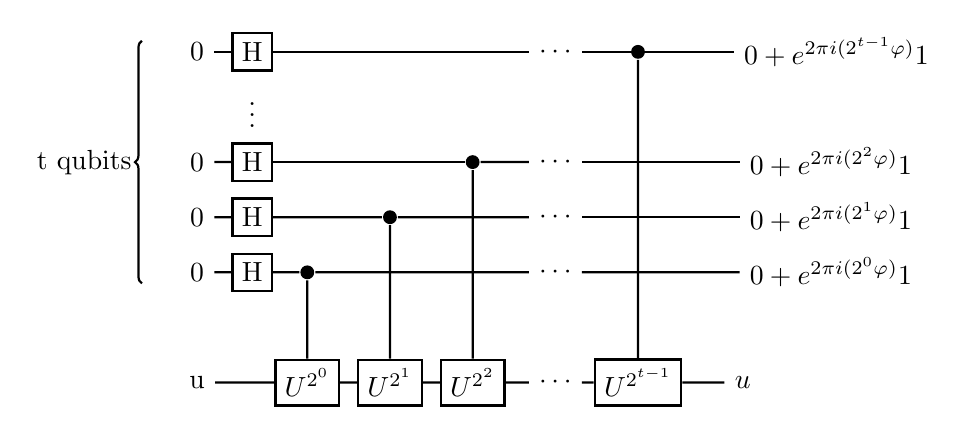
\begin{tikzpicture}[thick,scale=0.7]
        %
        % `operator' will only be used by Hadamard (H) gates here.
        % `phase' is used for controlled phase gates (dots).
        % `surround' is used for the background box.
        \tikzstyle{H} = [draw,fill=white,minimum size=1.2em] 
        \tikzstyle{U} = [draw,fill=white,minimum size=1.3em] 
        \tikzstyle{D} = [fill,shape=circle,minimum size=5pt,inner sep=0pt]
        %\tikzstyle{surround} = [fill=blue!10,thick,draw=black,rounded corners=2mm]
        
        % Bracket
        \draw[decorate,decoration={brace},thick] (-1,-4.2) -- node[left] {t qubits} (-1, 0.2);
        %\draw[decorate,decoration={brace},thick] (-1,-6.6) -- (-1, -5.4);

        % Column 0
        \node at (0,0)  (Q00) {\rs{0}}; 
        
        \node at (0,-2) (Q02) {\rs{0}}; 
        \node at (0,-3) (Q03) {\rs{0}}; 
        \node at (0,-4) (Q04) {\rs{0}}; 

        \node at (0,-6) (Q06) {\rs{u}}; 
        
 %      % Column 1
        \node[H] (H10) at (1,0) {H} edge [-] (Q00);
        \node    (D11) at (1,-1) {$\vdots $} ;
        \node[H] (H12) at (1,-2) {H} edge [-] (Q02);
        \node[H] (H13) at (1,-3) {H} edge [-] (Q03);
        \node[H] (H14) at (1,-4) {H} edge [-] (Q04);
 %
 %      % Column 2
        \node[D] (D24) at (2,-4) {} edge [-] (H14);
        \node[U] (U26) at (2,-6) {$U^{2^0}$} edge [-] (Q06);
        \draw[-] (D24) -- (U26);

 %
 %      % Column 3.5
        \node[D] (D33) at (3.5,-3) {} edge [-] (H13);
        \node[U] (U36) at (3.5,-6) {$U^{2^1}$} edge [-] (U26);
        \draw[-] (D33) -- (U36);

  %     % Column 5
        \node[D] (D52) at (5,-2) {} edge [-] (H12);
        \node[U] (U56) at (5,-6) {$U^{2^2}$} edge [-] (U36);
        \draw[-] (D52) -- (U56);%

        % Column 6.5

        \node (D60) at (6.5,0) {$\cdots$} edge [-] (H10);

        \node (D62) at (6.5,-2) {$\cdots$} edge [-] (D52);
        \node (D63) at (6.5,-3) {$\cdots$} edge [-] (D33);
        \node (D64) at (6.5,-4) {$\cdots$} edge [-] (D24);

        \node (D66) at (6.5,-6) {$\cdots$} edge [-] (U56);

        % Column 8 
        \node[D] (D80) at (8,0) {} edge [-] (D60);
        \node[U] (U86) at (8,-6) {$U^{2^{t-1}}$} edge [-] (D66);
        \draw[-] (D80) -- (U86);%
 
 %      % Column 9.5
        \node at (11.6,0)  (H90) {$\rs{0}+e^{2\pi i (2^{t-1} \varphi)} \rs{1}$} edge [-] (D60); 

        \node at (11.5,-2) (H92) {$\rs{0}+e^{2\pi i (2^{2} \varphi)} \rs{1}$} edge [-] (D62);  
        \node at (11.5,-3) (H93) {$\rs{0}+e^{2\pi i (2^{1} \varphi)} \rs{1}$} edge [-] (D63);  

        \node at (11.5,-4) (H94) {$\rs{0}+e^{2\pi i (2^{0} \varphi)} \rs{1}$} edge [-] (D64);  

        \node at (9.9,-6) (H96) {$\rs{u}$} edge [-] (U86);    

    \end{tikzpicture}
    }
    \end{figure}
\end{frame}

\begin{frame}
    {\Bullet}~受控U门的做作用效果, 作用到本征态$\rs{u}$,得到本征值 $e^{2\pi i \varphi}$ 
    \begin{itemize}
        \item $\rs{0}U\rs{u}=\rs{0}\rs{u}$
        \item $\rs{1}U\rs{u}=\rs{1} e^{2\pi i \varphi}\rs{u}$ 
    \end{itemize}
    {\Bullet}~线路工作原理 \\
    \begin{itemize}
        \item $H\rs{0}=\Pstate$
        \item $\Pstate U\rs{u}=\dfrac{1}{\sqrt{2}} (\rs{0}\rs{u} +  e^{2\pi i \varphi}\rs{1}\rs{u})= \dfrac{1}{\sqrt{2}} (\rs{0} +  e^{2\pi i \varphi}\rs{1})\rs{u} $ 
        \item $\Pstate U^{2^n}\rs{u}= \dfrac{1}{\sqrt{2}} (\rs{0} + e^{2\pi i (2^n \varphi)\rs{1} })\rs{u} $ 
    \end{itemize}
\end{frame}

\begin{frame}
    \frametitle{}
    {\Bullet}~混合之后,t-qubits为:
    \[ \dfrac{1}{\sqrt{2^t}} [\rs{0} + e^{2\pi i (2^{t-1} \varphi)\rs{1} }] [\rs{0} + e^{2\pi i (2^{t-2} \varphi)\rs{1} }]\cdots [\rs{0} + e^{2\pi i (2^0 \varphi)\rs{1} }] \]
    考虑到$\varphi$的二进制形式:
    \[\varphi=0.\varphi_1 \varphi_2 \cdots \varphi_t = \frac{\varphi_1}{2^1} + \frac{\varphi_2}{2^2}+\cdots + \frac{\varphi_t}{2^t}\]
    \[2^{t-1} \varphi= \varphi_1 \varphi_2 \cdots \varphi_{t-1}.\varphi_t=0.\varphi_t\]
    \[2^{t-2} \varphi= \varphi_1 \varphi_2 \cdots \varphi_{t-2}.\varphi_{t-1}\varphi_t=0.\varphi_{t-1}\varphi_t\]
    上式可写成
    \[ \dfrac{1}{\sqrt{2^t}} [\rs{0} + e^{2\pi i 0.\varphi_t)}\rs{1} ] [\rs{0} + e^{2\pi i 0.\varphi_{t-1}\varphi_t }\rs{1} ]\cdots [\rs{0} + e^{2\pi i 0.\varphi_1\varphi_2\cdots \varphi_t}\rs{1}] \]
    正是傅里叶变换乘积式! 
\end{frame}

\begin{frame}
    \frametitle{傅里叶反变换}
    以三量子比特线路为例:
    \tikzstyle{every picture}+=[remember picture]
    \begin{figure}
      \centerline{
        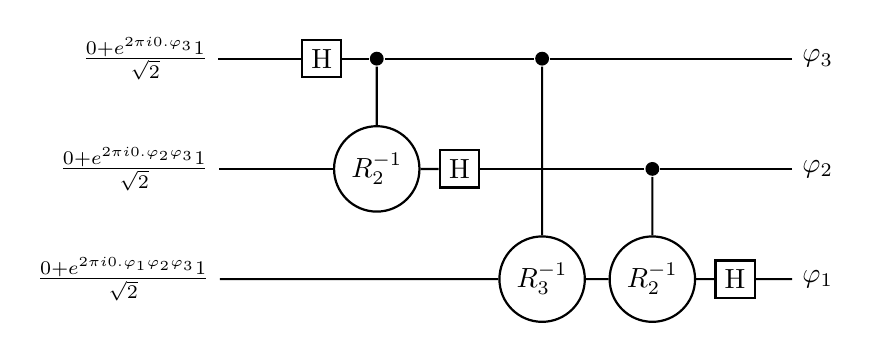
\begin{tikzpicture}[thick,scale=0.7]
        %
        % `operator' will only be used by Hadamard (H) gates here.
        % `phase' is used for controlled phase gates (dots).
        % `surround' is used for the background box.
        \tikzstyle{H} = [draw,fill=white,minimum size=1.2em] 
        \tikzstyle{U} = [draw,shape=circle,fill=white,minimum size=1.2em] 
        \tikzstyle{D} = [fill,shape=circle,minimum size=5pt,inner sep=0pt]
        %\tikzstyle{surround} = [fill=blue!10,thick,draw=black,rounded corners=2mm]
        
        % Bracket
        %\draw[decorate,decoration={brace},thick] (-1,-4.2) -- node[left] {t qubits} (-1, 0.2);
        %\draw[decorate,decoration={brace},thick] (-1,-6.6) -- (-1, -5.4);

        % Column 0
        \node at (-2.2,0)  (Q00) {$\frac{\rs{0}+e^{2\pi i 0.\varphi_3}\rs{1}}{\sqrt{2}}$}; 
        \node at (-2.4,-2) (Q01) {$\frac{\rs{0}+e^{2\pi i 0.\varphi_2\varphi_3}\rs{1}}{\sqrt{2}}$}; 
        \node at (-2.6,-4) (Q02) {$\frac{\rs{0}+e^{2\pi i 0.\varphi_1\varphi_2\varphi_3}\rs{1}}{\sqrt{2}}$}; 
        
 %      % Column 1
        \node[H] (H10) at (1,0) {H} edge [-] (Q00);
 %
 %      % Column 2
        \node[D] (D20) at (2,0) {} edge [-] (H10);
        \node[U] (U21) at (2,-2) {$R_2 ^{-1}$} edge [-] (Q01);
        \draw[-] (D20) -- (U21);

 %
 %      % Column 3.5
        \node[H] (H31) at (3.5,-2) {H} edge [-] (U21);

  %     % Column 5
        \node[D] (D50) at (5,0) {} edge [-] (D20);
        \node[U] (U52) at (5,-4) {$R_3 ^{-1}$} edge [-] (Q02);
        \draw[-] (U52) -- (D50);%

        % Column 6.5

        \node[D] (D61) at (7,-2) {} edge [-] (H31);
        \node[U] (U62) at (7,-4) {$R_2 ^{-1}$} edge [-] (U52);
        \draw[-] (D61) -- (U62);%

        % Column 8 
        \node[H] (H82) at (8.5,-4) {H} edge [-] (U62);

 
 %      % Column 9.5
        \node at (10,0)  (Q90) {$\rs{\varphi_3}$} edge [-] (D50); 
        \node at (10,-2)  (Q91) {$\rs{\varphi_2}$} edge [-] (D61);  
        \node at (10,-4)  (Q92) {$\rs{\varphi_1}$} edge [-] (H82); 
    \end{tikzpicture}
    }
    \end{figure}
\end{frame}


\begin{frame}
    \frametitle{推导}
    {\Bullet}~第一个量子比特过H门
    \begin{itemize}
        \item $\varphi_3=0; \quad \frac{\rs{0}+e^{2\pi i 0.\varphi_3}\rs{1}}{\sqrt{2}} = \Pstate; \quad H\Pstate = \rs{0} =\rs{\varphi_3} $
        \item $\varphi_3=1; \quad \frac{\rs{0}+e^{2\pi i /2 }\rs{1}}{\sqrt{2}} = \Mstate; \quad H\Mstate = \rs{1} =\rs{\varphi_3} $
    \end{itemize}
    总之
    \begin{itemize}
        \item $ H \frac{\rs{0}+e^{2\pi i 0.\varphi_3}\rs{1}}{\sqrt{2}} = \rs{\varphi_3}$
    \end{itemize}
\end{frame}

\begin{frame}
    \frametitle{}
    {\Bullet}~第二个量子比特过四分之一反转门
    \begin{itemize}
        \item $\varphi_3=0; \quad \frac{\rs{0}+e^{2\pi i 0.\varphi_2\varphi_3}\rs{1}}{\sqrt{2}} =  \frac{\rs{0}+e^{2\pi i 0.\varphi_2}\rs{1}}{\sqrt{2}} $
        \item $\varphi_3=1; \quad R_2 ^{-1} \frac{\rs{0}+e^{2\pi i 0.\varphi_2\varphi_3}\rs{1}}{\sqrt{2}} =  \frac{\rs{0}+e^{2\pi i 0.\varphi_2}\rs{1}}{\sqrt{2}} $
    \end{itemize}
    再过H门 
    \begin{itemize}
        \item $ H \frac{\rs{0}+e^{2\pi i 0.\varphi_2}\rs{1}}{\sqrt{2}} = \rs{\varphi_2}$
    \end{itemize}
\end{frame}

\begin{frame}
    \frametitle{}
    {\Bullet}~第三个量子比特过八分之一反转门
    \begin{itemize}
        \item $ R_3 ^{-1} \frac{\rs{0}+e^{2\pi i 0.\varphi_1\varphi_2\varphi_3}\rs{1}}{\sqrt{2}} =  \frac{\rs{0}+e^{2\pi i 0.\varphi_1\varphi_2}\rs{1}}{\sqrt{2}} $
    \end{itemize}
    过四分之一反转门
    \begin{itemize}
        \item $ R_2 ^{-1} \frac{\rs{0}+e^{2\pi i 0.\varphi_1\varphi_2}\rs{1}}{\sqrt{2}} =  \frac{\rs{0}+e^{2\pi i 0.\varphi_1}\rs{1}}{\sqrt{2}} $
    \end{itemize}
    再过H门 
    \begin{itemize}
        \item $ H \frac{\rs{0}+e^{2\pi i 0.\varphi_1}\rs{1}}{\sqrt{2}} = \rs{\varphi_1}$
    \end{itemize}
\end{frame}

\begin{frame}
    \frametitle{测量}
    {\Bullet}~测量 $\rs{\varphi_1},\rs{\varphi_2},\rs{\varphi_3} $\\\vspace{2em}
    获得相位$\varphi=0.\varphi_1\varphi_2\varphi_3$ \\ 


\end{frame}

\section{2.求本征值}

\begin{frame}
    \frametitle{求本征值}
    对于本征态,相位估计完成如下映射:
    \[\rs{0}\rs{u_k}\to F[\rs{\varphi_k}]\rs{u_k}\]
    对于任意态,有展开式
    \[\Psi=\sum_k \alpha_k \rs{u_k}\]
    相位估计完成映射
    \[\rs{0}\Psi = \sum_k \alpha_k \rs{0} \rs{u_k}\to \sum_k \alpha_k F[\rs{\varphi_k}]\rs{u_k}\]
    基此,可得到每一个本态的相位$\varphi_k$,及本征值$e^{2\pi i \varphi_k}$
\end{frame}


\section{3.大数质因式分解}

\begin{frame}
    \frametitle{因数分解}
    \例 [试问,下面这个数能不能做质因式分解]
    {\[N=39772916239307209103\]}
    \解~ (1)求$\sqrt{N}$,并取整$P=[\sqrt{N}]$ \\
    (2)求$N/P$,并取整$Q=[N/P]$ \\
    (3) 扫描 1-min(P,Q)之间的所有质数,判断是否存在两个质数$p,q$, 有
    \[p \times q = N\]
    工作量指数增长,当N很大时,目前的计算机就很难完成。\\
    相反,当我们知道$p=6257493337$时,就很容易验证$q=6356046119$ \\
    现化的密码学就是基于这个原理设计的。
\end{frame}

\begin{frame}
    \frametitle{阶的定义}
    量子算法,可以有效进行大数质因式分解,从而破解现有密码。\\
    基本思想为求阶!\\
    \begin{tcolorbox1}[0.86]{阶的定义}
    对于正整数x和N ($x\le N$),无公因子。则 x模N有阶r 定义为使
        \[x^r=1(mod N)\]
    成立的最小正整数。
    \end{tcolorbox1}  
\end{frame}

\begin{frame}
    \frametitle{}    
    \begin{columns}[T,onlytextwidth]
        \column{0.49\textwidth} 
        ~\\ \vspace{5em}
        \例 [试求x=11和N=21的阶r]{} 
        \解 (1) 取$r=1,2,3,\cdots$,依次计算 $11^r$ \\
        (2) 依次计算 $\dfrac{11^r}{21}$ 的余数\\
        (3) 第一个余数为1的r=6,得解\\ \vspace{2em}

        左表表明,阶就是余子式(完全集)的自由度
        \column{0.49\textwidth}
        \begin{center}
            \includegraphics[width=0.8\textwidth]{figs/38.png}
        \end{center}
    \end{columns}
\end{frame}

\begin{frame}
    \frametitle{}  
    \例 [试证明求阶问题与因式分解问题等价]{}  
    \证 设N可以作因子分解 $N=n_1\times n_2$
    若阶r为偶数,有
        \[x^r= 1 (mod N)\]
        \[x^r-1= M\times N \]
        \[(x^{r/2}-1) (x^{r/2}+1)=  M\times N = M\times n_1\times n_2 \]
    上式表明,求最大公约数
    \[gcd(x^{r/2}-1, N); \quad gcd(x^{r/2}+1, N)\]  
    很可能就能得到因子 $n_1$ 和 $n_2$ \\
    因此,因式分解问题就转化求阶问题,它们是等价的!
\end{frame}

\begin{frame}
    \frametitle{量子求阶}  
    \begin{itemize}
        \item 阶r就是余子式(完全集)的自由度。
        \item 量子傅里叶变换公式中,N就是基矢数目
        \[\boxed{y_k = \frac{1}{\sqrt{N}} \sum_{j=0} ^{N-1} x_j  e^{i \frac{2\pi}{N} jk} } \]
        \item 量子力学表明这个数目就是体系的自由度,即上式可取$N=r$
    \end{itemize}
    余子式$\{\rs{x^k~mod~N}\} $构成完全集,任意态函数可在其上展开,比如本征态S
    \[\rs{u_s} = \frac{1}{\sqrt{r}} \sum_{k=0} ^{r-1}  e^{-i \frac{2\pi}{r} sk} \rs{x^k~mod~N}  \]
\end{frame}

\begin{frame}
    \frametitle{}  
    对上式做傅里叶逆变换
    \[\rs{x^k~mod~N}   = \frac{1}{\sqrt{r}} \sum_{s=0} ^{r-1}  e^{-i \frac{2\pi}{r} sk} \rs{u_s} \]
    取k=0,得到余子式1态在量子本征函数系 $\{\rs{u_s}\}$的展开式
    \[\rs{x^0~mod~N}   =  \sum_{s=0} ^{r-1} \frac{1}{\sqrt{r}} \rs{u_s} =\sum_{s=0} ^{r-1} a_s \rs{u_s} \]
    其振幅(展开系数)$a_s=\dfrac{1}{\sqrt{r}}$,完全由阶(r)决定!  
\end{frame}

\begin{frame}
    \frametitle{求阶的算法推导} 
    \begin{center}
    \begin{tcolorbox1}[0.86]{$u_s$的本征值}
        试证明相位估计算子U的本征态$u_s$的本征值为$\exp[i2\pi\varphi]=\exp[i2\pi\frac{s}{r}]$
    \end{tcolorbox1}    
    \end{center}
 
     即要证明其本征方程为:
    \[U\rs{u_s}=\exp[i2\pi\frac{s}{r}] \rs{u_s}\]
\end{frame}

\begin{frame}
    \frametitle{}     
    \证~相位估计算子U在余子式有如下作用效果
    \[U\rs{y}=\rs{xy~\mod~N}\]
    \[\begin{aligned}
     \rs{u_s} &= \frac{1}{\sqrt{r}} \sum_{k=0} ^{r-1}  e^{-i \frac{2\pi}{r} sk} \rs{x^k \mod N}  \\
     U\rs{u_s} &= \frac{1}{\sqrt{r}} \sum_{k=0} ^{r-1}  e^{-i \frac{2\pi}{r} sk} U\rs{x^k \mod N}  \\
     &= \frac{1}{\sqrt{r}} \sum_{k=0} ^{r-1}  e^{-i \frac{2\pi}{r} sk} \rs{x^{k+1} \mod N}  \\
     &= \frac{1}{\sqrt{r}} \sum_{k'=1} ^{r}  e^{-i \frac{2\pi}{r} s(k'-1)} \rs{x^{k'} \mod N} 
    \end{aligned}\]   
\end{frame}

\begin{frame}
    \frametitle{}        
    \[\begin{aligned}
    &= \frac{1}{\sqrt{r}} e^{i \frac{2\pi}{r}s }  \sum_{k'=1} ^{r}  e^{-i \frac{2\pi}{r} sk' } \rs{x^{k'} \mod N} \\
    &= \frac{1}{\sqrt{r}} e^{i \frac{2\pi}{r}s }  \sum_{k'=1} ^{r-1}  e^{-i \frac{2\pi}{r} sk' } \rs{x^{k'} \mod N} 
    + \frac{1}{\sqrt{r}} e^{i \frac{2\pi}{r}s }  e^{-i \frac{2\pi}{r} s r } \rs{x^{r} \mod N} \\
    &= \frac{1}{\sqrt{r}} e^{i \frac{2\pi}{r}s }  \sum_{k'=1} ^{r-1}  e^{-i \frac{2\pi}{r} sk' } \rs{x^{k'} \mod N} 
    + \frac{1}{\sqrt{r}} e^{i \frac{2\pi}{r}s }  e^{-i 2\pi s } \rs{x^{0} \mod N} \\
    &= \frac{1}{\sqrt{r}} e^{i \frac{2\pi}{r}s }  \sum_{k'=0} ^{r-1}  e^{-i \frac{2\pi}{r} sk' } \rs{x^{k'} \mod N} \\
    &=\exp[i2\pi\frac{s}{r}] \rs{u_s}
    \end{aligned}\]  
    证毕! 
\end{frame}

\begin{frame}
    \frametitle{}  
    \[U\rs{u_s}=\exp[i2\pi\frac{s}{r}] \rs{u_s} = \exp[i2\pi\varphi] \rs{u_s}\]
    因此
    \[\varphi=\frac{s}{r}\]
    $\varphi$ 可通过傅里叶逆变换求得,则阶$r$可通过连分数算法求得
\end{frame}

\begin{frame}
    \frametitle{连分数算法}  
    \begin{center}
        \includegraphics[width=0.6\textwidth]{figs/39.png}
    \end{center}
    \begin{itemize}
        \item 有理数的连分数表示是有限的
        \item 任一有理数的连分数表示是唯一的
        \item “简单”有理数的连分数表示是简短的
        
    \end{itemize}  
\end{frame}

\begin{frame}
    \frametitle{}
    \begin{tcolorbox3}[专题、Grover量子搜索算法]
        (1)给出Grover算法量子线路 \\
        (2)推导算法过程\\
    \end{tcolorbox3}
\end{frame}  
%

%%%%%%%%%%%%%%%%%%%%%%%%%%%%%%%%%%%55%%
\begin{frame} [plain]
    \frametitle{}
    \Background[1] 
    \begin{center}
    {\huge 第8:量子通信(1)    }
    \end{center}  
    \addtocounter{framenumber}{-1}   
\end{frame}
%%%%%%%%%%%%%%%%%%%%%%%%%%%%%%%%%%

\section{1.量子通信基础}
\begin{frame}
    \frametitle{量子通信网络}
    \begin{center}
        \includegraphics[width=0.85\textwidth]{figs/40.png}
    \end{center}
\end{frame}

\begin{frame}
    \frametitle{经典香农熵}
    假设一个事件有N种可能的结果,对应的概率分布为$\{p_k\}$,则香农熵定义为:
    \[H(x)=\sum_{k=1}^{N} p_{k} \log _{2} \frac{1}{p_{k}} \text { (bit) }\]
    代表测得可获取信息量的平均值\\
    对于2态事件,有:
    \[\begin{aligned} H_{2} &=p_{0} \log _{2} \frac{1}{p_{0}}+p_{1} \log _{2} \frac{1}{p_{1}} \\ 
        &=p \log _{2} \frac{1}{p}+(1-p) \log _{2} \frac{1}{(1-p)} \\
        &=1; \quad \text{if} \quad p=\frac{1}{2}
     \end{aligned}\]   
\end{frame}

\begin{frame}
    \frametitle{量子Von Neumann熵}
    设体系第n个本征态出现的概率为$p_n$,则密度矩阵和熵分别定义为:
    \[\rho=\sum_{n=1} p_{n}|n\rangle\langle n| \]
    \[S(\rho)=-\operatorname{tr}\left(\rho \log _{2} \rho\right)\]
    对于双粒子体系:有
    \[S\left(\rho_{A B}\right)=-\operatorname{tr}\left(\rho_{A B} \log _{2} \rho_{A B}\right)\]
    \[S\left(\rho_{A} \otimes \rho_{B}\right)=S\left(\rho_{A}\right)+S\left(\rho_{B}\right)\]
    \[S\left(\rho_{A} ; \rho_{B}\right)=\left[S\left(\rho_{A}\right)+S\left(\rho_{B}\right)\right]-S\left(\rho_{A B}\right)\]
\end{frame}

\begin{frame}
    \frametitle{密钥密码体系}
    \begin{itemize}
        \item  原文: I love you
        \item  密文: M PSZI CSY
        \item  加码函数: $f(x)=x+\alpha \bmod 26$
        \item  解码函数: $f^{-1}(y)=y-\alpha \bmod 26$
        \Item  密钥:$\alpha=4$ \\
        \item  原文序列:abcd{\color{red}{e}}fgh{\color{red}{i}}jk{\color{red}{l}}mn{\color{red}{o}}pqrst{\color{red}{u}}{\color{red}{v}}wx{\color{red}{y}}z \\
        \item  密文序列:ab{\color{green}{c}}defgh{\color{green}{i}}jkl{\color{green}{m}}no{\color{green}{p}}qr{\color{green}{s}}tuvwx{\color{green}{y}}{\color{green}{z}} \\ \vspace{1em}
        请问有多少个可能密钥?
    \end{itemize}
\end{frame}

\begin{frame}
    \frametitle{单时拍密钥方案}
    \begin{itemize}
        \item 原文字符串长度为$n$ \[ a_1a_2a_3\ldots a_n\]
        \item 信息发送者制备一个长度也为$n$的密钥串 \[ b_1b_2b_3\ldots b_n\]
        \item 加密函数 \[ c_i=a_i+b_i \bmod N \]
        \item 密文串 \[ c_1c_2c_3\ldots c_n\]
        \item 解密函数 \[ a_i=c_i-b_i \bmod N \]
    \end{itemize}
\end{frame}

\begin{frame}
    \frametitle{公开钥密方案}
    \begin{itemize}
        \item RSA密码方案: R.L.Rivest,A.Shamir和 L.Adelman于1978年提出的
        \item 依据:“验证两个大素数容易,而将他们的乘积做因数分解则极其困难” 
        \item 原文: $X$
        \item 密文: $Y$
        \item 加密: 使用公钥($e,N$) $Y=X^{e} \bmod N$
        \item 解密:使用私钥($d,N$) $X=Y^{d} \bmod N$
    \end{itemize}
\end{frame}

\begin{frame}
    \frametitle{}
    {\color{red}{制备}}:(e,d,N)
    \begin{enumerate}
        \item 秘密选择两个大素数$p,q$
        \item 计算出$N=p\times q$
        \item 计算出欧拉函数$\Phi(N)=(p-1)\times (q-1)$
        \item 选择一个较小的素数$e$做为公钥,它与$\Phi(N)$互质
        \item 计算私钥$d$, $ed\equiv 1 \mod \Phi(N)$
    \end{enumerate}
     {\color{red}{破解}}:想从$e$得到$d$,必须知道$\Phi(N)$;想要得到$\Phi(N)$,必须知道$p,q$; 想要得到$p,q$,必须做大数质因式分解$N=p \times q$!
\end{frame}


\begin{frame}
    \frametitle{密钥分发}
    \begin{itemize}
        \Item 密使分发 $\qquad$ 怕汉奸!
        \Item 公开分发 $\qquad$ 怕量子算法!
    \end{itemize}
    必须发展量子算法破解不了的量子密钥公开分发方案!
\end{frame}

\section{2.量子密码分发~Quantum key Distribution}
\begin{frame}
    \frametitle{量子不可克隆原理}
    {\Bullet}~克隆(cloning)指在目标系统(B)中产生一个与源系统(A)相同的态,而不改变源系统的态。\\ \vspace{1em}
    \例[1.试证明未知量子态不可克隆]{}
    \证~设已知的本征态可以克隆
    \[ U_c\rs{C}\rs{0}_A\rs{\varphi}_B=\rs{C_0}\rs{0}_A\rs{0}_B\]
    \[ U_c\rs{C}\rs{1}_A\rs{\varphi}_B=\rs{C_1}\rs{1}_A\rs{1}_B\]
    若A处于未知叠加态\[ \rs{\Psi}_A=\alpha\rs{0}+\beta\rs{1}\]
\end{frame}

\begin{frame}
    \frametitle{}
    期望的克隆:
    \[\begin{aligned}
        U_{c}|C\rangle|\psi\rangle_{A}|\varphi\rangle_{B}=&\left|C_{\psi}\right\rangle|\psi\rangle_{A}|\psi\rangle_{B} \\
        =&\left.\left|C_{\psi}\right\rangle(\alpha|0\rangle+\beta)|1\rangle\right)_{A}(\alpha|0\rangle+\beta|1\rangle)_{B} \\
        =&\left|C_{\psi}\right\rangle\left(\alpha^{2}|0\rangle_{A}|0\rangle_{B}+\alpha \beta|0\rangle_{A}|1\rangle_{B}+\alpha \beta|1\rangle_{A}|0\rangle_{B}\right.\\
        &~~\left.+\beta^{2}|1\rangle_{A}|1\rangle_{B}\right)
        \end{aligned} 
    \]
     服从量子力学的过程:
    \[ \begin{aligned}
        U_{c}|C\rangle|\psi\rangle_{A}|\varphi\rangle_{B} &=U_{c}|C\rangle\left(\alpha|0\rangle+\beta|1\rangle\right)_{A}|\varphi\rangle_{B} \\
        &=U_{c}|C\rangle \alpha|0\rangle_{A}|\varphi\rangle_{B}+U_{c}|C\rangle \beta|1\rangle_{A}|\varphi\rangle_{B} \\
        &=\alpha^{2}\left|C_{0}\right\rangle|0\rangle_{A}|0\rangle_{B}+\beta^{2}\left|C_{1}\right\rangle|1\rangle_{A}|1\rangle_{B}
        \end{aligned}
    \]
    ~~\\
    两式相等的必要条件为 $\alpha\beta=0$, 即可克隆的$\rs{\Psi}_A$态不可能是叠加态!\\
    证毕!          
\end{frame}

\begin{frame}
    \frametitle{量子不可删除原理}
    {\Bullet}~删除是指如果目标系统(B)有源系统(A)的量子态副本,把B”置零” 而不改变A系统的状态
    \例[2.试证明未知量子态不可删除]{}
    \证~设已知的本征态可以删除
    \[ U_c\rs{C}\rs{0}_A\rs{0}_B=\rs{C_{00}}\rs{0}_A\rs{R}_B\]
    \[ U_c\rs{C}\rs{1}_A\rs{1}_B=\rs{C_{11}}\rs{0}_A\rs{R}_B\]
    \[ U_c\rs{C}\rs{0}_A\rs{1}_B=\rs{C_{01}}\rs{0}_A\rs{1}_B\]
    \[ U_c\rs{C}\rs{1}_A\rs{0}_B=\rs{C_{10}}\rs{0}_A\rs{0}_B\]
\end{frame}


\begin{frame}
    \frametitle{}
    对于叠加态,期望的删除:
    \[\begin{aligned}
        U_{c}|C\rangle|\psi\rangle_{A}|\psi\rangle_{B}&=\left|C_{\psi}\right\rangle|\psi\rangle_{A}|R\rangle_{B} \\
        &=|C_{\psi}\rangle(\alpha\rs{0}+\beta\rs{1})_{A}|R\rangle_{B} 
        \end{aligned} 
    \]
     服从量子力学的过程:
    \[ \begin{aligned}
        U_{c}|C\rangle|\psi\rangle_{A}|\psi\rangle_{B}=&U_{c}|C\rangle(\alpha|0\rangle+\beta|1\rangle)_{A}(|\alpha| 0\rangle+\beta|1\rangle)_{B} \\
        =& U_{c}|C\rangle \alpha^{2}|0\rangle_{A}|0\rangle_{B}+U_{c}|C\rangle \beta^{2}|1\rangle_{A}|1\rangle_{B} \\
        &~~+U_{c}|C\rangle \alpha \beta|0\rangle_{A}|1\rangle_{B}+U_{c}|C\rangle \alpha \beta|1\rangle_{A}|0\rangle_{B} \\
        =& \alpha^{2}\left|C_{00}\right\rangle|0\rangle_{A}|R\rangle_{B}+\beta^{2}\left|C_{11}\right\rangle|1\rangle_{A}|R\rangle_{B} \\
        &~~+\left|C_{01}\right\rangle \alpha \beta|0\rangle_{A}|1\rangle_{B}+\left|C_{10}\right\rangle \alpha \beta|1\rangle_{A}|0\rangle_{B}
        \end{aligned}
    \]
    ~~\\
    两式根本无法相等,即可删除的$\rs{\Psi}_A$态不可能是叠加态!\\
    证毕!          
\end{frame}

\subsection{BB84量子密码分发协议}
\begin{frame}
    \frametitle{}
    \begin{tcolorbox2}{BB84协议}
    {1984年,C. H. Bennett 和G. Brassard 提出利用偏振光进行量子密钥分发的协议。把一次性密码原理和量子测量原理结合在一起,建立不可破解密码分发方案}
    \end{tcolorbox2}  
\end{frame}

\begin{frame}
    \frametitle{原理}
    \begin{enumerate}
        \item Ailce 由随机数序列a决定选择纵横基还是对角基。设a中的0代表纵横基{$\rs{0},\rs{1}$},1代表对角基{$\rs{+},\rs{-}$} 
        \item Ailce 再由随机数序列a' 决定发射给Bob的光子的具体偏振。设a'中的0代表$\rs{0},\rs{+}$\\
        \hspace{2em} 设有 $a=0010$,$a'=1001$:Ailce发出的光子的偏振序列为$\rs{10+1}$
        \item Bob 得到偏振光子串后,由随机数序列b决定选择纵横基还是对角基,再由随机数序列b' 决定用相应基里的那个基矢波片进行测量\\
        \hspace{2em} 设有 $b=0110$,$b'=1100$:Bob使用的偏振片序列为$\rs{1-+0}$ 
        \item 双方公布第一序列(a=0010 and b=0110),发现第1、3位相同。
        \item 双方就知道各自手里的$a'=1001$和$b'=1100$中的第1、3位相同。整理出来,为$10$,并以此做为私钥d,完成密钥分发。
    \end{enumerate}
\end{frame}

\begin{frame}
    \frametitle{}
    {\color{red}{保密性分析}}:
    \begin{enumerate}
        \item 设有窃听者C,先得到A发给B的每一个光子。这阻断了A、B之间的通信,没有得到d。
        \item C想知道光子的状态,若测量,因不知道具体的基,导致每个光子有$50\%$概率状态改变。
        \item C因不知光子状态,不能进行克隆,强行克隆势必导致原光子状态改变。
        \item C只能窃听Ailce和Bob的通信,得到a和b,但不是a'和b'。
        \item 派内鬼分别去Ailce和Bob的办公室,窃取a'和b',难度大于窃取d。
    \end{enumerate}
\end{frame}

\begin{frame}
    \frametitle{}    
    \begin{columns}[T,onlytextwidth]
        \column{0.49\textwidth} 
        ~\\ \vspace{5em}
        \例 [试求x=11和N=21的阶r]{} 
        \解 (1) 取$r=1,2,3,\cdots$,依次计算 $11^r$ \\
        (2) 依次计算 $\dfrac{11^r}{21}$ 的余数\\
        (3) 第一个余数为1的r=6,得解\\ \vspace{2em}

        左表表明,阶就是余子式(完全集)的自由度
        \column{0.49\textwidth}
        \begin{center}
            \includegraphics[width=0.8\textwidth]{figs/38.png}
        \end{center}
    \end{columns}
\end{frame}

\begin{frame}
    \frametitle{}  
    \例 [试证明求阶问题与因式分解问题等价]{}  
    \证 设N可以作因子分解 $N=n_1\times n_2$
    若阶r为偶数,有
        \[x^r= 1 (mod N)\]
        \[x^r-1= M\times N \]
        \[(x^{r/2}-1) (x^{r/2}+1)=  M\times N = M\times n_1\times n_2 \]
    上式表明,求最大公约数
    \[gcd(x^{r/2}-1, N); \quad gcd(x^{r/2}+1, N)\]  
    很可能就能得到因子 $n_1$ 和 $n_2$ \\
    因此,因式分解问题就转化求阶问题,它们是等价的!
\end{frame}

\begin{frame}
    \frametitle{量子求阶}  
    \begin{itemize}
        \item 阶r就是余子式(完全集)的自由度。
        \item 量子傅里叶变换公式中,N就是基矢数目
        \[\boxed{y_k = \frac{1}{\sqrt{N}} \sum_{j=0} ^{N-1} x_j  e^{i \frac{2\pi}{N} jk} } \]
        \item 量子力学表明这个数目就是体系的自由度,即上式可取$N=r$
    \end{itemize}
    余子式$\{\rs{x^k~mod~N}\} $构成完全集,任意态函数可在其上展开,比如本征态S
    \[\rs{u_s} = \frac{1}{\sqrt{r}} \sum_{k=0} ^{r-1}  e^{-i \frac{2\pi}{r} sk} \rs{x^k~mod~N}  \]
\end{frame}

\begin{frame}
    \frametitle{}  
    对上式做傅里叶逆变换
    \[\rs{x^k~mod~N}   = \frac{1}{\sqrt{r}} \sum_{s=0} ^{r-1}  e^{-i \frac{2\pi}{r} sk} \rs{u_s} \]
    取k=0,得到余子式1态在量子本征函数系 $\{\rs{u_s}\}$的展开式
    \[\rs{x^0~mod~N}   =  \sum_{s=0} ^{r-1} \frac{1}{\sqrt{r}} \rs{u_s} =\sum_{s=0} ^{r-1} a_s \rs{u_s} \]
    其振幅(展开系数)$a_s=\dfrac{1}{\sqrt{r}}$,完全由阶(r)决定!  
\end{frame}

\begin{frame}
    \frametitle{求阶的算法推导} 
    \begin{center}
    \begin{tcolorbox1}[0.86]{$u_s$的本征值}
        试证明相位估计算子U的本征态$u_s$的本征值为$\exp[i2\pi\varphi]=\exp[i2\pi\frac{s}{r}]$
    \end{tcolorbox1}    
    \end{center}
 
     即要证明其本征方程为:
    \[U\rs{u_s}=\exp[i2\pi\frac{s}{r}] \rs{u_s}\]
\end{frame}

\begin{frame}
    \frametitle{}     
    \证~相位估计算子U在余子式有如下作用效果
    \[U\rs{y}=\rs{xy~\mod~N}\]
    \[\begin{aligned}
     \rs{u_s} &= \frac{1}{\sqrt{r}} \sum_{k=0} ^{r-1}  e^{-i \frac{2\pi}{r} sk} \rs{x^k \mod N}  \\
     U\rs{u_s} &= \frac{1}{\sqrt{r}} \sum_{k=0} ^{r-1}  e^{-i \frac{2\pi}{r} sk} U\rs{x^k \mod N}  \\
     &= \frac{1}{\sqrt{r}} \sum_{k=0} ^{r-1}  e^{-i \frac{2\pi}{r} sk} \rs{x^{k+1} \mod N}  \\
     &= \frac{1}{\sqrt{r}} \sum_{k'=1} ^{r}  e^{-i \frac{2\pi}{r} s(k'-1)} \rs{x^{k'} \mod N} 
    \end{aligned}\]   
\end{frame}

\begin{frame}
    \frametitle{}        
    \[\begin{aligned}
    &= \frac{1}{\sqrt{r}} e^{i \frac{2\pi}{r}s }  \sum_{k'=1} ^{r}  e^{-i \frac{2\pi}{r} sk' } \rs{x^{k'} \mod N} \\
    &= \frac{1}{\sqrt{r}} e^{i \frac{2\pi}{r}s }  \sum_{k'=1} ^{r-1}  e^{-i \frac{2\pi}{r} sk' } \rs{x^{k'} \mod N} 
    + \frac{1}{\sqrt{r}} e^{i \frac{2\pi}{r}s }  e^{-i \frac{2\pi}{r} s r } \rs{x^{r} \mod N} \\
    &= \frac{1}{\sqrt{r}} e^{i \frac{2\pi}{r}s }  \sum_{k'=1} ^{r-1}  e^{-i \frac{2\pi}{r} sk' } \rs{x^{k'} \mod N} 
    + \frac{1}{\sqrt{r}} e^{i \frac{2\pi}{r}s }  e^{-i 2\pi s } \rs{x^{0} \mod N} \\
    &= \frac{1}{\sqrt{r}} e^{i \frac{2\pi}{r}s }  \sum_{k'=0} ^{r-1}  e^{-i \frac{2\pi}{r} sk' } \rs{x^{k'} \mod N} \\
    &=\exp[i2\pi\frac{s}{r}] \rs{u_s}
    \end{aligned}\]  
    证毕! 
\end{frame}

\begin{frame}
    \frametitle{}  
    \[U\rs{u_s}=\exp[i2\pi\frac{s}{r}] \rs{u_s} = \exp[i2\pi\varphi] \rs{u_s}\]
    因此
    \[\varphi=\frac{s}{r}\]
    $\varphi$ 可通过傅里叶逆变换求得,则阶$r$可通过连分数算法求得
\end{frame}

\begin{frame}
    \frametitle{连分数算法}  
    \begin{center}
        \includegraphics[width=0.6\textwidth]{figs/39.png}
    \end{center}
    \begin{itemize}
        \item 有理数的连分数表示是有限的
        \item 任一有理数的连分数表示是唯一的
        \item “简单”有理数的连分数表示是简短的
        
    \end{itemize}  
\end{frame}  %                     %
%%%%%%%%%%%%%%%%%%%%%%%%%%%%%%%%%%%%%%%%%%%
\begin{frame}
    \frametitle{}
    \begin{center}
    { {\huge 第九讲、对易关系求解}}
    \end{center}    
\end{frame}
%%%%%%%%%%%%%%%%%%%%%%%%%%%%%%%%%%%%%


\section{前情回顾}

\begin{frame}
    \frametitle{前情回顾}
    \begin{itemize}
        \item 希尔伯特空间的态矢量描述体系状态
        \item 希尔伯特空间的算符给出体系的物理量
        \item 算符的本征函数系构成正交归一完全基
        \item 常见算符本征方程求解
    \end{itemize}   
\end{frame} 

\section{对易子及运算法则}
\begin{frame} 
    \frametitle{对易子定义}
    \begin{definition}
        定义对易子:$$ [F,G]\equiv FG-GF $$ \\
        若$[F,G]=0$,则对易 \\
        若$[F,G]\neq0$,则不对易
    \end{definition}
\end{frame} 

\begin{frame} 
    \frametitle{运算法则}
    \begin{enumerate}
        \item  $[A,B]=-[B,A]$
        \item  $[A,A]=0$
        \item  $[A,c]=0$
        \item  $[A,B+C]=[A,B]+[A,C]$
        \item  $[A,BC]=B[A,C]+[A,B]C$
        \item  $[AB,C]=A[B,C]+[A,C]B$
    \end{enumerate}
\end{frame} 
\begin{frame}
    \begin{proof}{}   
        \begin{equation*}
            \begin{split} 
            [AB,C]&=ABC-CAB \\
            A[B,C]+[A,C]B&=A(BC-CB)+(AC-CA)B\\
            &=ABC-ACB+ACB-CAB\\
            &=ABC-CAB
            \end{split}  
        \end{equation*}  
        $$ [AB,C]=A[B,C]+[A,C]B $$
    \end{proof}
\end{frame} 

\begin{frame} 
    \begin{tcolorbox}[colback=yellow!5,colframe=red!75!black,title=推论:]
        \begin{itemize}
            \item 如果A与B、C对易,则A与$B+C$对易
            \item 如果A与B、C对易,则A与$B^n+C^m$对易
            \item 如果A与B、C对易,则A与$BC$对易
            \item 如果A与B、C对易,则A与$B^nC^m$对易
            \item 如果A与B、C对易,则A与$B^nC^m+B^{n'}C^{m'}$对易
        \end{itemize}
    \end{tcolorbox}
\end{frame} 

\begin{frame} [allowframebreaks=]
    \begin{proof}{}
        \begin{equation*}
            \begin{split} 
             [A,B^{n}]&=[A,BB^{n-1}] \\
             &=B[A,B^{n-1}]+[A,B]B^{n-1}\\
             &=B[A,B^{n-1}] \\
             &=B^2[A,B^{n-2}]\\
             &=\cdots\\
             &=B^{n-1}[A,B]\\
             &= 0\\
            \end{split}  
        \end{equation*}  
    \end{proof}
    \begin{proof}{}
        同理:$[A,C^{m}]=0$\\
        \begin{equation*}
            \begin{split} 
            [A,B^{n}+C^{m}] &= [A,B^{n}]+[A,C^{m}]\\
            &=0 \\
            [A,B^{n}C^{m}] &= B^{n}[A,C^{m}] + [A,B^{n}] C^{m}\\
            &=0 \\
        \end{split}  
        \end{equation*}
        同理:$[A,B^{n'}C^{m'}]=0$\\
        \begin{equation*}
            \begin{split} 
            [A,B^{n}C^{m}+B^{n'}C^{m'}] &= [A,B^{n}C^{m}]+[A,B^{n'}C^{m'}]\\
            &=0\\
        \end{split}  
        \end{equation*}
    \end{proof}
\end{frame} 

\section{对易关系}
\begin{frame} [allowframebreaks=]
    \frametitle{1.位置-动量对易关系}
    \begin{exampleblock}{}
     求位置动量对易关系 $[x,p_x]=?$,  $[x,p_y]=?$
    \end{exampleblock}
    \alert{解:} 对任意波函数$\psi$,有
    \begin{equation*}
        \begin{split}
        xp_x\psi&= x(-i\hbar \frac{\partial}{\partial x})\psi \\
        &=-i\hbar x \frac{\partial}{\partial x}\psi\\
        p_x x \psi&= -i\hbar \frac{\partial}{\partial x} (x\psi) \\
        &=-i\hbar\psi - i\hbar x \frac{\partial}{\partial x}\psi \\
        \end{split}  
    \end{equation*}
    两式相减,$$(xp_x-p_x x)\psi= i\hbar\psi$$
    得 $xp_x-p_x x= i\hbar$ \\
    即 $[x,p_x]= i\hbar$\\
    同理,有:\\
    $\begin{cases}
        [x,p_x]= i\hbar  \\ 
        [y,p_y]= i\hbar  \\ 
        [z,p_z]= i\hbar  
    \end{cases}$
    $\begin{cases}
        [x,p_y]= 0  \\ 
        [y,p_z]= 0  \\ 
        [z,p_x]= 0  
    \end{cases}$
    $\begin{cases}
        [p_x,p_y]= 0  \\ 
        [p_y,p_z]= 0  \\ 
        [p_z,p_x]= 0  
    \end{cases}$
    $\begin{cases}
        [x,y]= 0  \\ 
        [y,z]= 0  \\ 
        [z,x]= 0  
    \end{cases}$ \\
    \begin{tcolorbox}[colback=yellow!5,colframe=red!75!black,title=量子力学基本对易关系]
    $\begin{cases}
        [x_\alpha,x_\beta]= 0  \\ 
        [p_\alpha,p_\beta]= 0  \\ 
        [x_\alpha,p_\beta]= i\hbar \delta_{\alpha\beta}  \\ 
    \end{cases}$
    \end{tcolorbox}
\end{frame} 

\begin{frame} [allowframebreaks=]
    \frametitle{2.角动量-位置}
    \begin{exampleblock}{}
     试证明角动量-位置对易关系 $[L_x,y]=i\hbar z,  [L_x,x]=0$
    \end{exampleblock}
    \alert{证明:} 
    \begin{equation*}
        \begin{split}
        [L_x,y]&= [yp_z-zp_y,y]\\
        &=-[y,yp_z-zp_y]\\
        &= -[y,yp_z] + [y,zp_y]\\
        &=-y[y,p_z] -[y,y]p_z + z[y,p_y] + [y,z]p_y\\
        &=-0 -0 + z i\hbar + 0\\
        &=i\hbar z \\
        \end{split}  
    \end{equation*}
    同理,有:\\
    $\begin{cases}
        [L_x,y]= i\hbar z  \\ 
        [L_x,x]= 0  \\ 
        [L_x,z]= -i\hbar y 
    \end{cases}$
    $\begin{cases}
        [L_y,z]= i\hbar x  \\ 
        [L_y,y]= 0  \\ 
        [L_y,x]= -i\hbar z 
    \end{cases}$
    $\begin{cases}
        [L_z,x]= i\hbar y  \\ 
        [L_z,z]= 0  \\ 
        [L_z,y]= -i\hbar x 
    \end{cases}$
    \begin{tcolorbox}[colback=yellow!5,colframe=red!75!black,title=角动量-位置对易关系]
        $$ [L_\alpha,x_\beta]= \varepsilon_{\alpha\beta\gamma} i\hbar x_\gamma $$ 
    \end{tcolorbox}
\end{frame} 

\begin{frame} [allowframebreaks=]
    \frametitle{3.角动量-动量}
    \begin{exampleblock}{}
     试证明角动量-动量对易关系 $[L_x,p_y]=i\hbar p_z,  [L_x,p_x]=0$
    \end{exampleblock}
    \alert{证明:} 
    \begin{equation*}
        \begin{split}
        [L_x,p_y]&= [yp_z-zp_y,p_y]\\
        &=-[p_y,yp_z-zp_y]\\
        &=-[p_y,yp_z] + [p_y,zp_y]\\
        &=-y[p_y,p_z] -[p_y,y]p_z + z[p_y,p_y] + [p_y,z]p_y\\
        &=-y[p_y,p_z] +[y,p_y]p_z + z[p_y,p_y] + [p_y,z]p_y\\
        &=-0 + i\hbar p_z + 0+0\\
        &=i\hbar p_z \\
        \end{split}  
    \end{equation*}
    同理,有:\\
    $\begin{cases}
        [L_x,p_y]= i\hbar p_z  \\ 
        [L_x,p_x]= 0  \\ 
        [L_x,p_z]= -i\hbar p_y 
    \end{cases}$
    $\begin{cases}
        [L_y,p_z]= i\hbar p_x  \\ 
        [L_y,p_y]= 0  \\ 
        [L_y,p_x]= -i\hbar p_z 
    \end{cases}$
    $\begin{cases}
        [L_z,p_x]= i\hbar p_y  \\ 
        [L_z,p_z]= 0  \\ 
        [L_z,p_y]= -i\hbar p_x 
    \end{cases}$
    \begin{tcolorbox}[colback=yellow!5,colframe=red!75!black,title=角动量-动量对易关系]
        $$ [L_\alpha,p_\beta]= \varepsilon_{\alpha\beta\gamma} i\hbar p_\gamma $$ 
    \end{tcolorbox}
\end{frame} 

\begin{frame} [allowframebreaks=]
    \frametitle{4.角动量-角动量}
    \begin{exampleblock}{}
     试证明位置角动量对易关系 $[L_x,L_y]=i\hbar L_z,  [L_z, L^2]= 0$
    \end{exampleblock}
    \alert{证明1:} 基于运算法则
    \begin{equation*}
        \begin{split}
        [L_x,L_y]= &[yp_z-zp_y,zp_x-xp_z]\\
        =&[yp_z,zp_x-xp_z] - [zp_y,zp_x-xp_z]\\
        =&y[p_z,zp_x-xp_z]+[y,zp_x-xp_z]p_z- z[p_y,zp_x-xp_z]-[z,zp_x-xp_z]p_y\\
        =&y[p_z,zp_x]-y[p_z,xp_z]+[y,zp_x]p_z-[y,xp_z]p_z \\ &-z[p_y,zp_x] +z[p_y,xp_z]- [z,zp_x]p_y+[z,xp_z]p_y\\
        =&yz[p_z,p_x]+y[p_z,z]p_x-yx[p_z,p_z]-y[p_z,x]p_z \\ & +z[y,p_x]p_z+[y,z]p_xp_z-x[y,p_z]p_z -[y,x]p_zp_z \\ & -zz[p_y,p_x] -z[p_y,z]p_x +zx[p_y,p_z] +z[p_y,x]p_z \\ & -z[z,p_x]p_y -[z,z]p_xp_y+x[z,p_z]p_y +[z,x]p_zp_y\\  
    \end{split}  
    \end{equation*}
    \begin{equation*}
        \begin{split}
        [L_x,L_y]=&0-yi\hbar p_x-0-0+0+0-0 -0-0 -0 +0 +0-0 -0+xi\hbar p_y +0\\
        =&i\hbar xp_y-i\hbar y p_x\\
        =&i\hbar (xp_y-y p_x)\\
        =&i\hbar L_z\\    
    \end{split}  
    \end{equation*}
    \alert{证明2:} 基于推论 
    \begin{equation*}
        \begin{split}
        [L_x,L_y]= &[yp_z-zp_y,zp_x-xp_z]\\
        =&[yp_z,zp_x-xp_z] - [zp_y,zp_x-xp_z]\\
        =&y[p_z,zp_x-xp_z]+[y,zp_x-xp_z]p_z- z[p_y,zp_x-xp_z]-[z,zp_x-xp_z]p_y\\
        =&y[p_z,zp_x]+0- 0-[z,-xp_z]p_y\\
        =&yz[p_z,p_x]+y[p_z,z]p_x+x[z,p_z]p_y+[z,x]p_zp_y\\
        =&0-yi\hbar p_x+x i\hbar p_y+0\\
        =&i\hbar L_z\\
    \end{split}  
    \end{equation*}
    同理,有:\\
    $\begin{cases}
        [L_x,L_y]= i\hbar L_z  \\ 
        [L_x,L_x]= 0  \\ 
        [L_x,L_z]= -i\hbar L_y 
    \end{cases}$
    $\begin{cases}
        [L_y,L_z]= i\hbar L_x  \\ 
        [L_y,L_y]= 0  \\ 
        [L_y,L_x]= -i\hbar L_z 
    \end{cases}$
    $\begin{cases}
        [L_z,L_x]= i\hbar L_y  \\ 
        [L_z,L_z]= 0  \\ 
        [L_z,L_y]= -i\hbar L_x 
    \end{cases}$
    \begin{tcolorbox}[colback=yellow!5,colframe=red!75!black,title=角动量对易关系]
        $$ [L_\alpha,L_\beta]= \varepsilon_{\alpha\beta\gamma} i\hbar L_\gamma $$ 
    \end{tcolorbox}
\end{frame} 

\begin{frame} [allowframebreaks=]
    \frametitle{}
    \begin{exampleblock}{}
     试证明角动量对易关系 $[L_z,L^2]=0$
    \end{exampleblock}
    \alert{证明:} 
    \begin{equation*}
        \begin{split}
        [L_z,L^2]&= [L_z,L_x ^2+L_y ^2+L_z ^2]\\
        &=[L_z,L_x ^2]+[L_z,L_y ^2]+[L_z,L_z ^2]\\
        &=[L_z,L_x ^2]+[L_z,L_y ^2]\\
        &=L_x[L_z,L_x] +[L_z,L_x]L_x +L_y[L_z,L_y] +[L_z,L_y]L_y\\
        &=i\hbar L_x L_y +i\hbar L_yL_x - i\hbar L_x L_y -i\hbar L_yL_x\\
        &=0 \\
        \end{split}  
    \end{equation*}
    同理,有:\\
    $\begin{cases}
        [L_x,L^2]= 0  \\ 
        [L_y,L^2]= 0  \\ 
        [L_z,L^2]= 0 
    \end{cases}$
    \begin{tcolorbox}[colback=yellow!5,colframe=red!75!black,title=角动量对易关系]
        $$ [L_\alpha,L^2]= 0 $$ 
    \end{tcolorbox}
\end{frame} 

\begin{frame} [allowframebreaks=]
    \frametitle{}
    \begin{tcolorbox}[colback=yellow!5,colframe=yellow!75!black,title=课堂作业]
        定义升降算符:$L_\pm \equiv L_x \pm i L_y$ \\
     试证明如下对易关系  $$[L_\pm,L^2]=0$$
     $$[L_z, L_\pm]= \pm \hbar L_\pm $$
     $$[L_+, L_-]= 2 \hbar L_z $$
    \end{tcolorbox}
\end{frame} 
  %   
%%%%%%%%%%%%%%%%%%%%%%%%%%%%%%%%%%%%%%%%%%%
\begin{frame}
    \frametitle{}
    \begin{center}
    { {\huge 第十讲、不确定性原理}}
    \end{center}    
\end{frame}
%%%%%%%%%%%%%%%%%%%%%%%%%%%%%%%%%%%%%


\section{前情回顾}

\begin{frame}
    \frametitle{前情回顾}
    \begin{itemize}
        \item 希尔伯特空间的态矢量描述体系状态
        \item 希尔伯特空间的算符给出体系的物理量
        \item 算符的本征函数系构成正交归一完全基
        \item 常见算符本征方程求解
        \item 算符对易关系求解
    \end{itemize}   
\end{frame} 

\section{对易的含义}
\begin{frame} 
    \frametitle{对易的含义}
    \begin{enumerate}
        \item  相互对易的两力学量算符,具有共同本征函数系
        \item  当体系处于共同的本征态时,它们同时具有确定值
        \item  构成最小完全集的一组力学量算符的数目等于体系的自由度。
    \end{enumerate}
\end{frame} 

\begin{frame} [allowframebreaks=]
    \begin{tcolorbox1}{定理1:}
        如果两算符具有共同的本征函数系,则它们对易
    \end{tcolorbox1}
    \alert{证明:} 设它们的共同本本征函数系为{$\varphi_n$}, 有:\\ 
        \begin{equation*}
            \begin{split} 
            A\varphi_n&=a_n \varphi_n \\
            B\varphi_n&=b_n \varphi_n \\
            \end{split}  
        \end{equation*}  
        对任意波函数
        \begin{equation*}
            \begin{split} 
            [A,B]\Psi &= [A,B]\sum_n c_n \varphi_n \\
            &= \sum_n c_n [A,B]\varphi_n \\
            &= \sum_n c_n (AB-BA)\varphi_n\\
            &= \sum_n c_n AB\varphi_n- \sum_n c_n BA\varphi_n\\
            &= \sum_n c_n a_nb_n\varphi_n- \sum_n c_n a_nb_n\varphi_n\\
            &=0\Psi
            \end{split}  
        \end{equation*}  
        得证: $$[A,B]=0$$
\end{frame} 

\begin{frame} [allowframebreaks=]
    \begin{tcolorbox1}{逆定理:}
       如果两算符对易,则它们具有共同的本征函数系。
    \end{tcolorbox1}
    \alert{证明:} 设A有本征函数系{$\varphi_n$}, 有:\\ 
        \begin{equation*}
            \begin{split} 
            A(B\varphi_n)&= AB\varphi_n\\
            &=BA\varphi_n \\
            &=Ba_n\varphi_n \\
            &=a_n(B\varphi_n) \\
            \end{split}  
        \end{equation*}  
        说明$B\varphi_n$ 和 $\varphi_n$ 都是A的属于本征值$a_n$的本征态,当$a_n$非简并时, 
        $B\varphi_n$ 和 $\varphi_n$ 描述同一个态,两者最多只差一个常数因子,记为 $b_n$,
        $$ B\varphi_n=b_n \varphi_n$$
        即: $\varphi_n$也是B的本征态。\\
        证毕!
\end{frame} 

\begin{frame} [allowframebreaks=]
    \begin{tcolorbox1}{推论1:}
        一组力学量算符具有共同本征函数完备系的充要条件是这些算符彼此两两对易
    \end{tcolorbox1}
    \alert{例子1:动量本征函数系} \\
    由于 $[p_\alpha,p_\beta]=0$,动量算符($p_x, p_y, p_z$)具有共同本征函数系 即平面波\\
    $$ \Psi_{\vec p}= \frac{1}{(2\pi\hbar)^{3/2}} e^{\frac{i}{\hbar}\vec{p}\cdot\vec{r}}$$ 
    \alert{例子2:角动量本征函数系} \\
    由于 $[L_z,L^2]=0$,它们具有共同的本征函数系 {$Y_{lm}$},\\
    当体系处于共同的本征态$Y_{lm}$时 ,它们同时具有确定值
    $$L_z= m\hbar, \qquad L^2=l(l+1)\hbar ^2 $$.
    当体系处于非共同的本征态,比如 $\frac{1}{\sqrt{2}}Y_{lm} + \frac{1}{\sqrt{2}}Y_{lm'}$,此时,$L^2$具有确定值
    $$L^2=l(l+1)\hbar ^2 $$,
    而$L_z$具有两个可能值(非确定)
    $$L_z= m\hbar\quad \text{or} \quad m'\hbar$$
    也就是说$\frac{1}{\sqrt{2}}Y_{lm} + \frac{1}{\sqrt{2}}Y_{lm'}$依然是$L^2$的本征态,却不是$L_z$的本征态。
\end{frame} 

\begin{frame} [allowframebreaks=]
    \begin{tcolorbox1}{推论2:}
        完全确定体系的一个量子态所需要的彼此对易的一组力学量算符集称为力学量完全集,最小力学量完全集所含力学量的数目等于体系的自由度。
    \end{tcolorbox1}
    \alert{例子1:空间的自由度为3} \\
    完全确定空间一个矢量(一个点)的位置,至少需要三个彼此对易的一组力学量构成的集,比如: $$(i,j,k) \qquad or \qquad (r,\theta,\varphi) $$
    当然,你可以用多于三个力学量构成的集来完全描述,但不是最小完全集!
    \alert{例子2:经典物理学} \\
    经典物理学用$\vec{r}, \vec{p}$来完全描述质点的运动状态,用了六个力学量$(x,y,z, p_x, p_y, p_z)$,量子力学发现这个集并不是彼此对易的,
    $$\begin{cases}
        [x_\alpha,x_\beta]= 0  \\ 
        [p_\alpha,p_\beta]= 0  \\ 
        [x_\alpha,p_\beta]= i\hbar \delta_{\alpha\beta}  \\ 
    \end{cases}$$
    它们不能构成一个完全集!
\end{frame} 

\section{不对易的含义}
\begin{frame} 
    \frametitle{不对易的含义}
    \begin{tcolorbox1}{不确定性原理:}
        两不对易力学量算符,一般不同时具有确定值    
    \end{tcolorbox1}
\end{frame} 

\begin{frame} 
    \frametitle{不确定度}
    \begin{itemize}
        \item 偏差: 测量值与平均值之差
        $$ \Delta F=F-\bar{F} $$
        \item 不确定度: 偏差的绝对值
         $$ \left | \Delta F  \right | $$
        \item 均方差: 偏差平方的平均值 (量子涨落)
        $$ \overline{(\Delta F)^2} = \overline{F^2} - \overline{F}^2$$
    \end{itemize}   
    我们通常先算(1)算符的平方的平均值和(2)算符的平均值平方,得到了均方差,再开方得到不确定度!
\end{frame} 


\begin{frame} 
    \frametitle{}
    \alert{证明:}
    \begin{equation*}
        \begin{split} 
        \overline{(\Delta F)^2}&= \overline{(F-\bar{F})^2}\\
        &=\overline{F^2-2F\bar{F}+\bar{F}^2 }\\
        &=\overline{F^2} -2\overline{F\bar{F}} +\overline{\bar{F}^2 }\\
        &=\overline{F^2} -2\overline{F}^2 +\overline{F}^2\\
        &= \overline{F^2} - \overline{F}^2
        \end{split}  
    \end{equation*} 
\end{frame} 

\begin{frame} 
    \frametitle{}
    \begin{tcolorbox2}{不确定度对易关系}
     试证明:  $$[\Delta F, \Delta G]= [F, G]$$
    \end{tcolorbox2}
    \alert{证明:}
    \begin{equation*}
        \begin{split} 
        [\Delta F, \Delta G]&= \Delta F \Delta G - \Delta G \Delta F \\
        &=(F-\bar{F}) (G-\bar{G})- (G-\bar{G}) (F-\bar{F}) \\
        &=FG -F\bar{G}-\bar{F}G + \bar{F} \bar{G} -GF + G \bar{F} + \bar{G} F -\bar{G} \bar{F}   \\
        &=FG-GF \\
        &=[F, G]
        \end{split}  
    \end{equation*} 
\end{frame} 

\begin{frame} [allowframebreaks=]
    \frametitle{}
    \alert{不确定性原理的严格证明:} \\
    令 $[\hat{F}, \hat{G}]= i\hat{k}$,对任意波函数,计算含实参$\xi$的积分:
    $$
    \begin{aligned}
    I(\xi)= &\int|(\xi\Delta \hat{F}-i \Delta \hat{G}) \psi|^{2} d \tau \quad (\geq 0) \\
    =&\int[\xi \Delta \hat{F} \psi-i \Delta \hat{G} \psi][\xi \Delta \hat{F} \psi-i \Delta \hat{G} \psi]^{*} d \tau \\
    =&\int[\xi \Delta \hat{F} \psi-i \Delta \hat{G} \psi] [\xi(\Delta \hat{F} \psi)^{*}+i(\Delta \hat{G} \psi)^{*}] d \tau \\
    =&\int[\xi \Delta \hat{F} \psi-i \Delta \hat{G} \psi]\left[\xi(\Delta \hat{F} \psi)^{*}+i(\Delta \hat{G} \psi)^{*}\right] d \tau \\
    =& \xi^{2} \int(\Delta \hat{F} \psi)(\Delta \hat{F} \psi) * d \tau-i \xi \int(\Delta \hat{G} \psi)(\Delta \hat{F} \psi) * d \tau \\
        &+i \xi \int(\Delta \hat{F} \psi)(\Delta \hat{G} \psi) * d \tau+\int(\Delta \hat{G} \psi)(\Delta \hat{G} \psi) * d \tau \\
    \end{aligned}
    $$
    $$
    \begin{aligned}
    =& \xi^{2} \int \psi^{*}(\Delta \hat{F})^{2} \psi d \tau-i \xi \int \psi^{*}(\Delta \hat{F} \Delta \hat{G}) \psi d \tau \\
    &+i \xi \int \psi^{*}(\Delta \hat{G} \Delta \hat{F}) \psi d \tau+\int \psi^{*}(\Delta \hat{G})^{2} \psi d \tau \\
    =& \xi^{2} \int \psi^{*}(\Delta \hat{F})^{2} \psi d \tau-i \xi \int \psi^{*}(\Delta \hat{F} \Delta \hat{G}-\Delta \hat{G} \Delta \hat{F}) \psi d \tau+\int \psi^{*}(\Delta \hat{G})^{2} \psi d \tau \\
    =& \xi^{2} \overline{(\Delta F)^{2}}-i \xi \overline{[\Delta F, \Delta G]}+\overline{(\Delta G)^{2}}\\
    =&\xi^{2} \overline{(\Delta F)^{2}}+\xi \overline{[F, G]}+\overline{(\Delta G)^{2}} \\
    =&\xi^{2} \overline{(\Delta F)^{2}}+\xi \bar{\hat{k}}+\overline{(\Delta G)^{2}} \\
    \geq & 0\\
    \end{aligned}
    $$
    对比不等式条件:
    $$
    a \xi^{2}+b \xi+c \geq 0
    $$
    $$
    b^{2}-4 a c \leq 0 \Rightarrow a c \geq \frac{b^{2}}{4}
    $$
    可知: 
    $$
    \overline{(\Delta \hat{F})^{2}} \cdot \overline{(\Delta \hat{G})^{2}} \geq \frac{(\bar{\hat{k}})^{2}}{4}
    $$
    得: 
    $$
    \overline{(\Delta \hat{F})^{2}} \cdot \overline{(\Delta \hat{G})^{2}} \geq \frac{1}{4}|\overline{[\hat{F}, \hat{G}]}|^{2}
    $$
    证毕!
\end{frame} 

\begin{frame}

$$ [x,p_x]=i\hbar $$
$$
\overline{(\Delta \hat{x})^{2}} \cdot \overline{(\Delta \hat{p_x})^{2}} 
\geq \frac{1}{4}|\overline{[\hat{x}, \hat{p_x}]}|^{2}=\frac{\hbar^2}{4}
$$
$$
\sqrt{\overline{(\Delta x)^{2}} \cdot \overline{(\Delta p_x)^{2}}} 
\geq \frac{\hbar}{2}
$$
$$  
\Delta x \cdot \Delta p_x 
\geq \frac{\hbar}{2}
$$ 
得位置-动量不确定性关系,称为海森堡不确定性关系.
\end{frame}

\begin{frame}
    \frametitle{海森堡}
    \begin{wrapfigure} {r} {0.3\textwidth} %;图在右
        \includegraphics[width=0.25\textwidth]{figs/hesb.png}   
    \end{wrapfigure}
    维尔纳·海森堡(Werner Heisenberg,1901年12月5日-1976年2月1日),德国物理学家,1932年诺贝尔物理学奖。主要贡献:(1) 创立矩阵力学(量子力学的矩阵形式);(2)提出“测不准原理”;(3)散射(S)矩阵。  
\end{frame}

\begin{frame}
    \frametitle{}
    \begin{center}
    \includegraphics[width=0.8\textwidth]{figs/uncert.png}
    \end{center}
\end{frame}


\begin{frame} [allowframebreaks=]
    \begin{tcolorbox2}{不确定性关系式表明:}
    \begin{itemize}
        \item 若两个力学量算符不对易(对易子不等于零),对易子平均值的平方一般大于零,则它们的不确定度的积必大于零,说明它们一般不能同时具有确定值
        \item 若两个力学量算符对易,则总可以找出这样的态(比如共同的本征态),使它们同时有确定值。 
    \end{itemize}   
    \end{tcolorbox2}
\end{frame} 

\begin{frame} [allowframebreaks=]
    TIPS:下列说法,正确的有:
    \begin{enumerate}
        \item 两力学量算符对易,则同时有确定值。 
        \item 两力学量算符不对易,则不能同时有确定值 
        \item 若两力学量算符有共同的本征态,则彼此对易
        \item 若两力学量算符不对易,则没有共同本征态
        \item 若[A,B]=常数,则A和B能有共同本征态
    \end{enumerate} 
\end{frame} 

\begin{frame} [allowframebreaks=]
    \frametitle{}
    \begin{tcolorbox}[colback=yellow!5,colframe=yellow!75!black,title=课堂作业]
    已知$[L_x, L_y]=i\hbar L_z$, 试计算体系处于$L_z$基态($Y_{00}=\frac{1}{\sqrt{4\pi}}$)时,$L_x, L_y$的不确定度。
    \end{tcolorbox}
\end{frame} 

  %  
%%%%%%%%%%%%%%%%%%%%%%%%%%%%%%%%%%%%%%%%%%%
\begin{frame}
    \frametitle{}
    \begin{center}
    { {\huge 第十一讲、对称与守恒量}}
    \end{center}    
\end{frame}
%%%%%%%%%%%%%%%%%%%%%%%%%%%%%%%%%%%%%


\section{前情回顾}

\begin{frame}
    \frametitle{前情回顾}
    \begin{itemize}
        \item 希尔伯特空间的态矢量描述体系状态
        \item 希尔伯特空间的算符给出体系的物理量
        \item 算符的本征函数系构成正交归一完全基
        \item 常见算符本征方程求解
        \item 算符对易关系及其物理含义 
    \end{itemize}   
\end{frame} 

\section{守恒量}
\begin{frame} 
    \frametitle{守恒量定义}
    \begin{enumerate}
        \item  经典物理中的守恒量与对称条件\\
                守恒量:力学量的值不随时间变化\\
                \begin{itemize}
                    \item 机械能空间平移不变→动量守恒
                    \item 机械能空间转动不变→角动量守恒
                    \item 机械能时间平移不变→能量守恒
                \end{itemize}
        \item  量子力学中的守恒量\\
                守恒量:在任意态下力学量的平均值不随时间变化\\
                $$ \bar{A}(t)=(\Psi(t), A\Psi(t)) =c.  $$
                守恒量及守恒条件... 
    \end{enumerate}
\end{frame} 



  %                     %
%\include{lecture12.tex}  % 
%%%%%%%%%%%%%%%%%%%%%%%%%%%%%%%%%%%%%%%%%%%
\begin{frame}
    \frametitle{}
    \begin{center}
    { {\huge 第十三讲、量子力学公式的矩阵化}}
    \end{center}    
\end{frame}
%%%%%%%%%%%%%%%%%%%%%%%%%%%%%%%%%%%%%

\section{前情回顾}


\begin{frame}
    \frametitle{前情回顾}
    \begin{itemize}
       \done 波函数矩阵表示 :$$ a_n(t)=(u_n(\vec{r}), \Psi(\vec{r},t)) $$ 
       \done 力学量算符矩阵表示 : $$ F_{nm}=(u_n (\vec{r}), Fu_m(\vec{r})) $$   
       \todo 公式的矩阵化:$\cdots$
    \end{itemize}
\end{frame} 



\begin{frame} 
    \frametitle{}
    \begin{tcolorbox}[colback=yellow!5,colframe=yellow!75!black,title=量子力学常用公式]
        \begin{itemize}
            \item 平均值公式
            \item 归一化公式
            \item 本征方程
            \item 薛定谔方程
            \item 运动方程
        \end{itemize}   
    \end{tcolorbox}
\end{frame} 

\section{平均值公式}

\begin{frame} 
    \frametitle{}
    \begin{tcolorbox}[colback=yellow!5,colframe=yellow!75!black,title=1、平均值公式]
        求平均值公式在Q表象中的具体形式(矩阵表示)
        $$ \bar{F}=\int \Psi^* (\vec{r},t) F \Psi(\vec{r},t) d\tau $$
    \end{tcolorbox}
    \alert{解:} 
    \begin{equation*}
        \begin{split}
            \bar{F}&=(\Psi(\vec{r},t), F\Psi(\vec{r},t)) \\
            &= (\sum_n a_n(t) u_n(\vec{r}), \sum_m a_m(t) F u_m(\vec{r}))\\
            &= \sum_{n,m} a_n ^*(t) (u_n(\vec{r}), F u_m(\vec{r})) a_m(t)\\
            &= \sum_{n,m} a_n ^*(t) F_{nm} a_m(t)\\
        \end{split} 
    \end{equation*}
\end{frame}

\begin{frame} 
    取遍$n, m$, 得到如下矩阵形式\\
    $$\bar{F} =(a_1 ^*(t), a_2 ^*(t),\cdots,a_n^*(t) )
    \begin{pmatrix}
       F_{11} & F_{12} & \cdots & F_{1n} \\
       F_{21} & F_{22} & \cdots & F_{2n} \\
       \cdots & \cdots &  \cdots& \cdots\\
        F_{n1} & F_{n2} & \cdots & F_{nn} \\
    \end{pmatrix}
    \begin{pmatrix}
        a_1(t)\\
        a_2(t)\\
        \cdots \\
        a_n(t)
    \end{pmatrix}
    $$ \vspace{1.0em} 
    $$ \large \color{red} \bar{F} = \pmb {\Psi} ^{\dagger } \pmb {F} \pmb {\Psi} $$
\end{frame}

\begin{frame} 
    在自身表象中,有:
    $$\bar{F} =(a_1 ^*(t), a_2 ^*(t),\cdots,a_n^*(t) )
    \begin{pmatrix}
       f_1 & 0 & \cdots & 0 \\
       0& f_2 & \cdots & 0 \\
       \cdots & \cdots &  \cdots& \cdots\\
        0 & 0 & \cdots & f_n \\
    \end{pmatrix}
    \begin{pmatrix}
        a_1(t)\\
        a_2(t)\\
        \cdots \\
        a_n(t)
    \end{pmatrix}
    $$
    \vspace{1.0em} 
    $$ \large \color{red} \bar{F} = \sum_n a_n^*(t) a_n(t) f_n= \sum_n |a_n(t)|^2 f_n $$
\end{frame}

\section{归一化公式}

\begin{frame} 
    \frametitle{}
    \begin{tcolorbox}[colback=yellow!5,colframe=yellow!75!black,title=2、归一化公式]
        求归一化公式在Q表象中的具体形式(矩阵表示)
        $$ \int \Psi^* (\vec{r},t) \Psi(\vec{r},t) d\tau =1 $$
    \end{tcolorbox}
    \alert{解:} 
    \begin{equation*}
        \begin{split}
            1 &=(\Psi(\vec{r},t), \Psi(\vec{r},t)) \\
            &= (\sum_n a_n(t) u_n(\vec{r}), \sum_m a_m(t) u_m(\vec{r}))\\
            &= \sum_{n,m} a_n ^*(t) (u_n(\vec{r}), u_m(\vec{r})) a_m(t)\\
            &= \sum_{n,m} a_n ^*(t) \delta_{nm} a_m(t)\\
        \end{split} 
    \end{equation*}
\end{frame}


\begin{frame} 
    $$  \sum_{n} a_n ^*(t) a_n(t) =1 $$
    取遍$n$, 得到如下矩阵形式\\
    $$ (a_1 ^*(t), a_2 ^*(t),\cdots,a_n^*(t) )
    \begin{pmatrix}
        a_1(t)\\
        a_2(t)\\
        \cdots \\
        a_n(t)
    \end{pmatrix}
    =1 $$ \vspace{1.0em} 
    $$ \large \color{red} \pmb {\Psi} ^{\dagger } \pmb {\Psi} =1 $$

\end{frame}

\section{本征方程}

\begin{frame} 
    \frametitle{}
    \begin{tcolorbox}[colback=yellow!5,colframe=yellow!75!black,title=3、本征方程]
        求本征方程在Q表象中的具体形式(矩阵表示)
        $$ F\psi_n (\vec{r}) =f \psi_n (\vec{r})$$
    \end{tcolorbox}
    \alert{解:} 
    \begin{equation*}
        \begin{split}
            F\psi_m (\vec{r}) &=f \psi_m \\
            \psi_n ^*  F\psi_m &=\psi_n ^* f \psi_m\\
            (\psi_n, F\psi_m )&=(\psi_n, f \psi_m)\\
            (\psi_n, F\psi_m )&=(\psi_n, f \psi_m)\\
            F_{nm} &=f_m \delta_{nm}
        \end{split} 
    \end{equation*}
\end{frame}

\begin{frame} 
    $$ \sum_n (F_{nm} -f \delta_{nm})a_n=0 $$
    取遍$n,m$, 得矩阵形式\\            
    $$\begin{pmatrix}
        F_{11}-f & F_{12} & \cdots & F_{1n} \\
        F_{21} & F_{22}-f & \cdots & F_{2n} \\
        \cdots & \cdots &  \cdots& \cdots\\
         F_{n1} & F_{n2} & \cdots & F_{nn}-f \\
     \end{pmatrix}
     \begin{pmatrix}
         a_1(t)\\
         a_2(t)\\
         \cdots \\
         a_n(t)
     \end{pmatrix}
     =0 \qquad (1)$$
     $$ \color{red} (\pmb F -f \pmb I) \pmb \Psi =0 $$

    有解条件,系数行列式等于零!
\end{frame}

\begin{frame} 
    得久期方程:
    $$\begin{vmatrix}
        F_{11}-f & F_{12} & \cdots & F_{1n} \\
        F_{21} & F_{22}-f & \cdots & F_{2n} \\
        \cdots & \cdots &  \cdots& \cdots\\
         F_{n1} & F_{n2} & \cdots & F_{nn}-f \\
     \end{vmatrix} 
     =0 \qquad (2) $$
     解久期方程, 得本征谱{$f_1,f_2,\cdots, f_n $}\\
     依次把$f_i$ 代回方程(1),解得第i个本征函数。本征方程得解\\
     矩阵化使本征方程从微分方程变为代数方程!
\end{frame}

\begin{frame} 
    \begin{tcolorbox}[colback=yellow!5,colframe=yellow!75!black,title=例1]
        已知算符在Q表象中的矩阵形式如下。
        $$ L_x= \frac{\hbar}{\sqrt{2}}
        \begin{pmatrix}
            0 & 1 & 0  \\
            1 & 0 & 1  \\
            0 & 1 & 0 \\
         \end{pmatrix} $$
        求本征值和归一化本征函数,并将矩阵对角化。
    \end{tcolorbox}
    可选方案:
    \begin{itemize}
        \done 解久期方程,得本征值,然后代入方程(1),得本征函数 ,再直接写出对角阵 
        \todo 直接从数学上对角化,对角元就是本征值,然后代入方程(1),得本征函数。
     \end{itemize}
\end{frame}

\begin{frame} 
    \alert{解:}第一步:解久期方程求本征值
    $$\frac{\hbar}{\sqrt{2}}
    \begin{vmatrix}
       0-f & 1 & 0  \\
       1 & 0-f & 1  \\
       0 & 1 & 0-f \\
    \end{vmatrix} 
    =0 \qquad (2) $$
   $$ -f^3+2f=0 $$
   $$ f_1=\sqrt{2}, f_2=0, f_3=-\sqrt{2} $$
   注意:这只是
   $$\begin{pmatrix}
       0 & 1 & 0  \\
       1 & 0 & 1  \\
       0 & 1 & 0 \\
    \end{pmatrix} $$
    的本征值,$L_x$的本征值为 $\lambda_i=\dfrac{\hbar}{\sqrt{2}} f_i$,即 $ \hbar, 0, -\hbar$
\end{frame}

\begin{frame} 
    第二步:把$f_i$ 代回方程(1)求本征函数
    $$\begin{pmatrix}
        0-f & 1 & 0  \\
        1 & 0-f & 1  \\
        0 & 1 & 0-f \\
     \end{pmatrix} 
     \begin{pmatrix}
         a_1\\
         a_2\\
         a_3
     \end{pmatrix}
     =0 \qquad (1)$$

     $$\begin{matrix}
       f_1=\sqrt{2} & f_2=0  &  f_3=-\sqrt{2}\\
    \begin{pmatrix}
        1/\sqrt{2}a_2\\
        a_2\\
        1/\sqrt{2}a_2
    \end{pmatrix}  
    = 1/\sqrt{2}a_2 \begin{pmatrix}
        1\\
        \sqrt{2}\\
        1
        \end{pmatrix} 
    & 
    \begin{pmatrix}
        a_1\\
        0\\
        a_1
    \end{pmatrix}  
    =  a_1 \begin{pmatrix}
        1\\
        0\\
        1
    \end{pmatrix}
    &
    \begin{pmatrix}
        -1/\sqrt{2}a_2\\
        a_2\\
        -1/\sqrt{2}a_2
    \end{pmatrix} 
    = 1/\sqrt{2}a_2 \begin{pmatrix}
        -1\\
        \sqrt{2}\\
        -1
    \end{pmatrix} 
    \end{matrix}$$           
\end{frame}


\begin{frame} 
    代入归一化公式, $$ \pmb {\Psi} ^{\dagger } \pmb {\Psi} =1 $$

    $$\begin{matrix}
    f_1=\sqrt{2} & f_2=0  &  f_3=-\sqrt{2}\\
    \dfrac{1}{2} a_2 ^2 (1, \sqrt{2}, 1)
    \begin{pmatrix}
    1\\
    {\sqrt{2}}\\
    1
    \end{pmatrix} 
    =1 
    & 
    a_1 ^2 (1, 0, 1)
    \begin{pmatrix}
     1\\
     0\\
     1
    \end{pmatrix} 
    =1 
     &
     \dfrac{1}{2} a_2 ^2 (-1, \sqrt{2}, -1)
    \begin{pmatrix}
     -1\\
     {\sqrt{2}}\\
     -1
    \end{pmatrix} 
    =1 \\
    a_2= \dfrac{1}{\sqrt{2}} &  a_1= \dfrac{1}{\sqrt{2}} &   a_2=\dfrac{1}{\sqrt{2}} 
    \\
    \psi_1=\dfrac{1}{2}
    \begin{pmatrix}
    1\\
    \sqrt{2}\\
    1
    \end{pmatrix}  
    & 
    \psi_2=\dfrac{1}{\sqrt{2}}
    \begin{pmatrix}
    1\\
    0\\
    1
    \end{pmatrix}  
    &
    \psi_3=\dfrac{1}{2}
    \begin{pmatrix}
    -1\\
    \sqrt{2}\\
    -1
    \end{pmatrix}  
    \end{matrix}$$   
\end{frame}

\begin{frame} 
    第三步:写出对角阵:
    $$ L_x= \frac{\hbar}{\sqrt{2}}
        \begin{pmatrix}
            0 & 1 & 0  \\
            1 & 0 & 1  \\
            0 & 1 & 0 \\
         \end{pmatrix} 
    = 
    \begin{pmatrix}
        \hbar & 0 & 0  \\
        0 & 0 &   \\
        0 & 0 & -\hbar \\
     \end{pmatrix} 
    $$
\end{frame}

\section{薛定谔方程}
\begin{frame} 
    \frametitle{}
    \begin{tcolorbox}[colback=yellow!5,colframe=yellow!75!black,title=4、薛定谔方程]
        求薛定谔方程在Q表象中的具体形式(矩阵表示)
        $$ i\hbar \frac{\partial}{\partial t }\psi (\vec{r},t) =H\psi (\vec{r},t)$$
    \end{tcolorbox}
    \alert{解:} 波函数在Q表象展开
    \begin{equation*}
        \begin{split}
            i\hbar \frac{\partial}{\partial t }\sum_n a_n(t) u_n(\vec{r})  &=H\sum_n a_n(t) u_n(\vec{r}) \\
            u_m ^* (\vec{r}) i\hbar \frac{\partial}{\partial t }\sum_n a_n(t) u_n(\vec{r})  &=u_m ^* (\vec{r})H\sum_n a_n(t) u_n(\vec{r}) \\
            i\hbar \frac{\partial}{\partial t }u_m ^* (\vec{r}) \sum_n a_n(t) u_n(\vec{r})  &=u_m ^* (\vec{r})\sum_n a_n(t) Hu_n(\vec{r}) \\      
        \end{split} 
    \end{equation*}
\end{frame}

\begin{frame} 
    \begin{equation*}
        \begin{split}
            i\hbar \frac{\partial}{\partial t }(u_m (\vec{r}), \sum_n a_n(t) u_n(\vec{r}) ) &=(u_m (\vec{r}), \sum_n a_n(t) Hu_n(\vec{r})) \\
            i\hbar \frac{\partial}{\partial t }\sum_n a_n(t)(u_m (\vec{r}),  u_n(\vec{r}) ) &=\sum_n (u_m (\vec{r}),  Hu_n(\vec{r}))a_n(t) \\
            i\hbar \frac{\partial}{\partial t }\sum_n a_n(t)\delta_{mn} &=\sum_n  H_{mn} a_n(t) \\
            i\hbar \frac{\partial}{\partial t } a_n(t) &=\sum_n H_{mn} a_n(t)  \\
        \end{split} 
    \end{equation*}
\end{frame}

\begin{frame} 
    取遍$n,m$, 得矩阵形式\\ 
    $$i\hbar \frac{\partial}{\partial t }  
    \begin{pmatrix}
        a_1(t)\\
        a_2(t)\\
        \cdots \\
        a_n(t)
    \end{pmatrix}
    =         
    \begin{pmatrix}
        H_{11} & H_{12} & \cdots & H_{1n} \\
        H_{21} & H_{22} & \cdots & H_{2n} \\
        \cdots & \cdots &  \cdots& \cdots\\
        H_{n1} & F_{n2} & \cdots & H_{nn} \\
     \end{pmatrix}
     \begin{pmatrix}
         a_1(t)\\
         a_2(t)\\
         \cdots \\
         a_n(t)
     \end{pmatrix}
    $$ \vspace{0.6em }
    $$\color{red} i\hbar \frac{\partial}{\partial t }  \pmb \Psi = \pmb H  \pmb \Psi $$
\end{frame}

\section{算符运动方程}
\begin{frame} 
    \frametitle{}
    \begin{tcolorbox}[colback=yellow!5,colframe=yellow!75!black,title=5、算符运动方程]
        求运动方程在Q表象中的具体形式(矩阵表示)
        $$ \frac{d\overline{F}}{dt}=\overline{\frac{\partial F }{\partial t}}  +\frac{1}{i\hbar} \overline{[F,H]}$$
    \end{tcolorbox}
    \alert{解:} 波函数在Q表象展
    \begin{equation*}
        \begin{split}
            \frac{d(\psi,F \psi )}{dt} &=(\psi,\frac{\partial F }{\partial t} \psi)  +\frac{1}{i\hbar}  ( \psi,[F,H]\psi) \\
            \frac{d(\sum_m a_m u_m,F \sum_n a_n u_n )}{dt} &=(\sum_m a_m u_m,\frac{\partial F }{\partial t} \sum_n a_n u_n) \\  
            &+\frac{1}{i\hbar}  (\sum_m a_m u_m,[F,H]\sum_n a_n u_n)  \\    
        \end{split} 
    \end{equation*}
\end{frame}

\begin{frame} 
    \begin{equation*}
        \begin{split}
            \frac{d\sum_{mn}a_m ^* (u_m,Fu_n )a_n}{dt} &=\sum_{mn} a_m ^*  (u_m,\frac{\partial F }{\partial t} u_n)a_n \\  
            &+\frac{1}{i\hbar} \sum_{mn} a_m ^*  ( u_m,[F,H] u_n)a_n  \\  
            \frac{d\sum_{mn}a_m ^* F_{mn}a_n}{dt} &=\sum_{mn} a_m ^*  \frac{\partial F_{mn} }{\partial t}a_n \\  
            &+\frac{1}{i\hbar} \sum_{mn} a_m ^* [F_{mn},H_{mn}]a_n  \\       
        \end{split} 
    \end{equation*}
\end{frame}

\begin{frame} 
    取遍$n,m$, 得矩阵形式
    \begin{equation*}
        \begin{split} 
            \frac{d \pmb \Psi^{\dagger } \pmb F \pmb \Psi}{dt} &=\pmb \Psi^{\dagger } \frac{\partial \pmb F }{\partial t} \pmb \Psi +\frac{1}{i\hbar} \pmb \Psi^{\dagger } [\pmb F, \pmb H] \pmb \Psi \\ \vspace{0.6em}  
           \color{red} \frac{d \overline{\pmb F}}{dt} & \color{red} =\overline{\frac{\partial \pmb F }{\partial t}} +\frac{1}{i\hbar} \overline{ [\pmb F,\pmb H]} \\      
        \end{split} 
    \end{equation*}
\end{frame}

\begin{frame} 
    \frametitle{}
    \begin{tcolorbox}[colback=yellow!5,colframe=yellow!75!black,title=课堂作业]
    取Q表象为动量表象,试求平均值公式和薛定谔方程的具体形式。
    \end{tcolorbox}
\end{frame}   %    
%\include{lecture14.tex}  %   
%%%%%%%%%%%%%%%%%%%%%%%%%%%%%%%%%%%%%%%%%%%
\begin{frame}
    \frametitle{}
    \begin{center}
    { {\huge 第十五讲、狄拉克(Dirac)符号}}
    \end{center}    
\end{frame}
%%%%%%%%%%%%%%%%%%%%%%%%%%%%%%%%%%%%%

\section{前情回顾}

\begin{frame}
    \frametitle{前情回顾}
    \begin{itemize}
       \done 波动力学
       \done 矩阵力学
       \todo 两者的统一 
    \end{itemize}
        \begin{center}
            \includegraphics[width=0.9\textwidth]{figs/2021-12-06-16-22-39.png}\\   
        \end{center}    
\end{frame} 

\section{狄拉克(Dirac)符号}

\begin{frame}
    量子力学用希尔伯特空间描述,希尔伯特空间是内积空间
    \begin{tcolorbox1}{希尔伯特空间}
    \begin{itemize}
        \item 加法:$\psi + \varphi$
        \item 数乘:$c\psi$
        \item 内积:$(\psi,\psi)$
    \end{itemize}
    \end{tcolorbox1}
    考察内积: $(\psi,\psi)=\int\psi^*\psi d\tau$ \\
    同一波函数放在左边还是右边,意义有所不同: \\
    放右边是线性矢量:  $(\psi,a\psi)=a (\psi,\psi)$ \\
    放左边是反线性矢量:   $(a\psi,\psi)=a^* (\psi,\psi)$   
\end{frame}

\begin{frame}
    \frametitle{1、左矢和右矢}
    \begin{tcolorbox1}{定义:}
    为了清楚地描述这种线性反线性特点,特定义左矢和右矢
    $$\langle \psi |, \qquad |\psi \rangle $$ 
    有 : $$\langle a\psi | = \langle \psi |a^* $$
    $$ |a\psi \rangle = a|\psi \rangle$$ 
    \end{tcolorbox1}
\end{frame} 

\begin{frame}
    \frametitle{}
    考察加法和数乘:发现其中的矢量通常是线性的,因此用右矢来代替。\\
    $$\begin{aligned}
    &\text{内积:}   & (\psi,\Psi)  & \qquad\Leftrightarrow \qquad & | \Psi \rangle =\langle \psi | \Psi \rangle \\
    &\text{平均值:}   & \bar{F}=(\Psi,F\Psi)  & \qquad\Leftrightarrow \qquad & \bar{F} =\langle \Psi|F | \Psi \rangle \\
    &\text{态叠加原理:}   & \Psi=a_1 \psi_1+ a_2 \psi_2  & \qquad\Leftrightarrow \qquad &| \Psi \rangle =a_1 |1 \rangle+ a_2 |2 \rangle\\
    &\text{展开式1:}     & \Psi=\sum\limits_{i=1} ^n a_i \psi_i & \qquad \Leftrightarrow \qquad &| \Psi \rangle =\sum\limits_{i=1} ^n a_i |i \rangle\\
    &\text{展开式2:}     & \Psi=\sum\limits_{i=1} ^n (\psi_i ,\Psi) \psi_i & \qquad \Leftrightarrow \qquad &| \Psi \rangle =\sum\limits_{i=1} ^n \langle i | \Psi \rangle |i\rangle\\
    \end{aligned}
    $$
\end{frame} 
 

\begin{frame}
    \frametitle{2、外积}
    考察展开式:
    $$\begin{aligned}
    \Psi \rangle &= \sum\limits_{i=1} ^n \langle i | \Psi \rangle |i\rangle\\
                 &= \sum\limits_{i=1} ^n |i\rangle\langle i | \Psi \rangle \\
    \end{aligned}
    $$
    定义算符: $ \qquad  \rho_i = |i\rangle\langle i | \qquad $ 有: \\
    $$\sum\limits_{i=1} ^n |i\rangle\langle i = \sum\limits_{i=1} ^n \rho_i =1 $$

\end{frame} 

\begin{frame}
    \frametitle{外积矩阵表示}
    若:$ \Psi =\sum a_n \varphi_n $\\
    右矢的矩阵形式:
    $$|\Psi\rangle = \begin{pmatrix}
        a_1\\
        a_2\\\
        \cdots\\
        a_n\
    \end{pmatrix}$$ 
    左矢的矩阵形式:
    $$ \langle\Psi| = (a_1 ^*, a_2 ^*, \cdots, a_n ^*) $$
    内积与外积:
    $$\langle\Psi|\Psi\rangle= (a_1 ^*, a_2 ^*, \cdots, a_n ^*) \begin{pmatrix}
        a_1\\
        a_2\\\
        \cdots\\
        a_n\
    \end{pmatrix},\qquad  |\Psi\rangle\langle\Psi|= \begin{pmatrix}
        a_1\\
        a_2\\\
        \cdots\\
        a_n\
    \end{pmatrix} (a_1 ^*, a_2 ^*, \cdots, a_n ^*) $$
\end{frame} 


\begin{frame}
    \frametitle{3、密度算符}
    算符的意义:
    $$\rho_i\Psi= |i\rangle\langle i | \Psi \rangle = \langle i | \Psi \rangle |i\rangle=a_i |i\rangle $$
    $$\Psi= \sum\limits_i ^n a_i |i\rangle = \sum\limits_i ^n \rho_i\Psi$$
    可知: $ \rho_i\Psi $ 是矢量$\Psi$ 在第$i$ 个本征矢上的投影, 因此称为{\color{red} 投影算符}\\
    对于非本征态,也可定义:$\rho = |\Psi\rangle\langle \Psi |$\\
    考察其在$i$态的平均值:
    $$ \begin{aligned}
    \bar{\rho} &=\langle i |\rho | i \rangle \\
               &=\langle i |\Psi\rangle\langle \Psi | i \rangle \\
               &=(\langle i |\Psi\rangle) (\langle \Psi | i \rangle) \\
               &=a_i ^* a_i =\omega_i \\
    \end{aligned} $$
    是概率密度,因此称 $\rho = |\Psi\rangle\langle \Psi |$ 为 {\color{red} 密度算符},也称为测量算符。
\end{frame} 
 
\begin{frame}
    \frametitle{4、密度矩阵}
    考察平均值公式:\\
    $$ \begin{aligned}
    \bar{\hat{F}} &=\sum\limits_i |a_i|^2 f_i \\
            &=\sum\limits_i \omega_i \langle i |\hat{F}|i \rangle  \\
            &=\sum\limits_{ij} \omega_i \langle i |\hat{F} |j\rangle \langle j| i\rangle  \\
            &=\sum\limits_{ij} \langle j| i\rangle  \omega_i \langle i |\hat{F} |j\rangle  \\
            &=\sum\limits_{j} \langle j | (\sum\limits_{i}| i \rangle  \omega_i \langle i |) \hat{F} |j\rangle  \\
    \end{aligned} $$
    定义密度矩阵:
    $$ \hat{\rho} = \sum\limits_{i}| i \rangle  \omega_i \langle i | $$
\end{frame} 
 
\begin{frame}  
    \frametitle{}  得新的平均公式:
    \begin{tcolorbox1}{平均公式-3}
         $$ \begin{aligned}
            \bar{\hat{F}}&=\sum\limits_{j} \langle j | \hat{\rho} \hat{F} |j\rangle \\
                &=tr (\hat{\rho} \hat{F} )
        \end{aligned} $$   
    \end{tcolorbox1} 
\end{frame} 
 
\begin{frame}      
    例:求算符$\hat{F}$在 $|\Psi\rangle =\sum\limits_n a_n |n\rangle $上的平均值 \\
    \alert{解:} 先求算符矩阵:
    $$ F_{nm} = \langle n | F |m \rangle  $$
    再求密度矩阵:
    $$ \hat{\rho} = \sum\limits_{n}| n \rangle  a_n ^* a_n \langle n | $$
    对两矩阵的积求迹得平均值
    $$\bar{\hat{F}}=tr (\hat{\rho} \hat{F} )$$
\end{frame} 
 
\begin{frame}  [allowframebreaks=]
    \frametitle{6、狄拉克型量子力学}  
    量子态: $\hspace{1em}|\Psi \rangle, \qquad$ 位置波函数:$\hspace{1em} \langle x |\Psi \rangle$ \\ \vspace{0.2em}
    展开式: $\hspace{1em}|\Psi \rangle =\sum\limits_{n=1} ^n a_n |n \rangle$ \\
    内积:   $\hspace{2em}\langle \varphi | \Psi \rangle = (\varphi, \Psi)= \int \varphi^*\Psi d\tau $ \\  \vspace{0.2em}
    归一化: $\hspace{1em}\langle \Psi | \Psi \rangle = (\Psi, \Psi)= \int \Psi^*\Psi d\tau = 1 $ \\ \vspace{0.2em}
    正交归一: $\langle n | m \rangle = \delta_{nm} $ \\ \vspace{0.2em}
    $ \hspace{5em} \langle \lambda | \lambda' \rangle = \delta(\lambda-\lambda') $\\ \vspace{0.2em}
    表象: $\hspace{2em}\Psi(x)= \langle x | \Psi \rangle$ \\ \vspace{0.2em}
    展开系数: $ a_n= \langle n | \Psi \rangle$ \\ \vspace{0.2em}
    展开系数: $ a_n ^*= \langle \Psi | n \rangle$ \\ \vspace{0.2em}
    平均值:  $\hspace{1em}\bar{F} = \langle \Psi |F | \Psi \rangle$ \\ \vspace{0.2em}
    矩阵元:  $\hspace{1em}F_{nm} = \langle n |F | m \rangle$ \\ \vspace{0.2em}
    本征方程:$F|n\rangle =f_n |n\rangle$ \\ \vspace{0.2em}
    幺正变换:$S_{m\alpha} =\langle m| \alpha \rangle $ \\ \vspace{0.2em}
    密度算符:$\rho = |\Psi\rangle\langle \Psi | $ \\ \vspace{0.2em}
    密度矩阵: $\hat{\rho} = \sum\limits_{i}| i \rangle  \omega_i \langle i | $ \\ \vspace{0.2em}
    薛定谔方程:$$ i\hbar \frac{\partial }{\partial t} |\Psi(t)\rangle = H|\Psi(t)\rangle $$ 
    算符运动方程:$$ \frac{d\bar{A}(t)}{dt}=\overline{(\frac{\partial A(t) }{\partial t})}  +\frac{1}{i\hbar} \overline{[A(t),H(t)]}$$
\end{frame} 
 
\begin{frame} 
    \frametitle{8、应用实例}  
    1、求波函数的矩阵表示:  
    $$|\Psi \rangle =\sum\limits_{n=1} ^n a_n |n \rangle$$
    $$ a_n= \langle n | \Psi \rangle$$ 
    展开系数构成矩阵表示:  
    $$\begin{pmatrix}
    a_1\\
    a_2\\\
    \cdots\\
    a_n\
    \end{pmatrix} $$
\end{frame} 

\begin{frame} 
    \frametitle{}  
    2、求算符的矩阵表示:  
    $$|\varphi \rangle = F |\Psi \rangle$$
    $$|\varphi \rangle = \sum_n F |n\rangle\langle n |\Psi \rangle$$
    $$\langle m |\varphi \rangle = \sum_n  \langle m| F |n\rangle\langle n |\Psi \rangle$$
    $$ b_m = \sum_n  F_{mn} a_n$$

    取遍$n,m$:  
    $$\begin{pmatrix}
    b_1\\
    b_2\\\
    \cdots\\
    b_n\
    \end{pmatrix} 
    = 
    \begin{pmatrix}
        F_{11} & F_{12} & \cdots & F_{1n} \\
        F_{21} & F_{22} & \cdots & F_{2n} \\
        \cdots & \cdots &  \cdots &  \cdots \\
        F_{n1} & F_{n2} & \cdots & F_{nn} \\
    \end{pmatrix} 
    \begin{pmatrix}
        a_1\\
        a_2\\\
        \cdots\\
        a_n\
    \end{pmatrix} 
    $$
\end{frame} 

\begin{frame} 
    3、求薛定谔方程的矩阵表示: 
    $$ \begin{aligned}
    i \hbar \frac{\partial}{\partial t} |\Psi \rangle &= H |\Psi \rangle  \\
    i \hbar \frac{\partial}{\partial t} \langle m |\Psi \rangle &= \langle m |H |\Psi \rangle \\ 
     &= \sum_n \langle m |H |n\rangle\langle n |\Psi \rangle  \\
     i \hbar \frac{\partial}{\partial t} a_m  &= \sum_n H_{mn} a_n 
    \end{aligned}
    $$
\end{frame} 

\begin{frame} 
    4、求平均值公式的矩阵表示: 
    $$ \begin{aligned}
    \bar{F} &= \langle \Psi |F |\Psi \rangle  \\
    &= \langle \Psi |1 \cdot F \cdot 1 |\Psi \rangle  \\
    &= \sum_{mn} \langle \Psi |m\rangle\langle m |F| n\rangle\langle n |\Psi \rangle  \\
    &= \sum_{mn} a_m ^* F_{mn} a_n 
    \end{aligned}
    $$
\end{frame} 

\begin{frame} 
    5、求两算符积的平均值: 
    $$ \begin{aligned}
    \overline{GF} &= \langle \Psi |GF |\Psi \rangle  \\
    &= \langle \Psi |1 \cdot G \cdot 1 \cdot F \cdot 1 |\Psi \rangle  \\
    &= \sum_{mln} \langle \Psi |m\rangle\langle m |G |l\rangle\langle l| F| n\rangle\langle n |\Psi \rangle  \\
    &= \sum_{mln} a_m ^* G_{ml} F_{ln} a_n 
    \end{aligned}
    $$
\end{frame} 

\section{量子力学绘景(Pictures)}

\begin{frame}  
    \frametitle{三种绘景}  
    \begin{enumerate}
        \item 薛定谔方程:$$ i\hbar \frac{\partial }{\partial t} |\Psi(t)\rangle = H|\Psi(t)\rangle $$
        \item 算符运动方程:$$ \frac{d\bar{A}(t)}{dt}=\overline{(\frac{\partial A(t) }{\partial t})}  +\frac{1}{i\hbar} \overline{[A(t),H(t)]}$$
    \end{enumerate}
    这个世界到底什么在变?\\
    \begin{itemize}
        \done 薛定谔绘景:只有波函数(态)在变,服从薛定谔方程
        \done 海森堡绘景:只有算符(力学量)在变,服从算符运动方程(海森堡方程)
        \done 狄拉克绘景:波函数和算符都在变,一切都只是幺正变换。
    \end{itemize}
\end{frame} 

\begin{frame}  
    \frametitle{}  
    定义时间演化算符:
    $$ U(t,t_0) |\Psi(t_0)\rangle = |\Psi(t)\rangle  $$
    \alert{分析}:
    (1) 因为 $ U(t_0,t_0) |\Psi(t_0)\rangle = |\Psi(t_0)\rangle  $ \\
     有:$$ U(t_0,t_0)=I $$
    (2):求 $ U(t,t_0)$
    $$ \begin{aligned}
        i\hbar \frac{\partial }{\partial t} |\Psi(t)\rangle &= H|\Psi(t)\rangle  \\
        i\hbar \frac{\partial }{\partial t}  U(t,t_0) |\Psi(t)\rangle &= H U(t,t_0) |\Psi(t)\rangle  \\
        i\hbar \frac{\partial }{\partial t}  U(t,t_0)  &= H U(t,t_0)  \\
        U(t,t_0)  &= e^{-\frac{i}{\hbar} H(t-t_0)}  \\
    \end{aligned} $$
\end{frame} 

\begin{frame}  
    (3):$ U(t,t_0)$是幺正算符
    $$ \begin{aligned}
        U(t,t_0)  &= e^{-\frac{i}{\hbar} H(t-t_0)}  \\
        U^\dagger (t,t_0)  &= e^{\frac{i}{\hbar} H(t-t_0)}  \\
        U^\dagger (t,t_0)U(t,t_0) &= U^\dagger (t,t_0)U(t,t_0) \\
         &=e^{\frac{i}{\hbar} H(t-t_0)-\frac{i}{\hbar} H(t-t_0)} \\
         &=e^0
         &=I
    \end{aligned} $$
    因此,有:
    $$ |\Psi(t)\rangle = U(t,t_0) |\Psi(t_0)\rangle   $$
    对比: 
    $$ |\psi_{(B)}\rangle = S^\dagger |\psi_{(A)}\rangle $$
    可知,波函数随时间的演化服从薛定谔方程,但也只是一种幺正算符。
\end{frame} 

\begin{frame}  
    \frametitle{} 
    (4)分析平均值公式:
    $$ \begin{aligned}
        \bar{F} &= \langle \Psi(t) |F(t_0) | \Psi \rangle(t)  \\
        &= \langle \Psi(t_0) |U^\dagger (t,t_0) |F(t_0) | U(t,t_0) |\Psi(t_0)\rangle   \\
        &= \langle \Psi(t_0) |U^\dagger (t,t_0) F(t_0) U(t,t_0) |\Psi(t_0)\rangle   \\
        &= \langle \Psi(t_0) F(t,t_0) |\Psi(t_0)\rangle   \\
    \end{aligned} $$
     式中,令: $$ F(t,t_0) =U^\dagger (t,t_0) F(t_0) U(t,t_0)$$
     对式:
     $$F'=S^\dagger F S $$
     可知,算符随时间的演化与波函数随时间的演化是等价的,也只是一种幺正算符。
\end{frame} 

\begin{frame}
    \frametitle{}  
    \centering
    \LARGE \color{red} 期中考试! \\
\end{frame}  %  
%-----------------------------------------------%

\begin{frame}
    \frametitle{}
    \centering {\color{red} {\textbf{\Huge A $\&$ Q}}}   
\end{frame} 

\end{document}